\documentclass[titlepage]{article}
\usepackage{amsmath}
\usepackage{amssymb}
\usepackage{indentfirst}
\usepackage[margin=1in]{geometry}
\usepackage{longtable}
\usepackage{enumitem}
\usepackage{fancyvrb}
%\usepackage{graphicx}
\usepackage{pdfpages}
\usepackage{subcaption}
\usepackage{flafter}
\usepackage[section]{placeins}
\usepackage{float}
\hyphenation{wave-guide}
\renewcommand\_{\textunderscore\linebreak[1]}

\begin{document}

\begin{titlepage}

   \centering
   \vspace*{3cm}
   {\huge\bfseries OpenParEMg User's Manual} \\
   \vskip1cm
   {\Large Version 1.0} \\
   \vskip1cm
   {\Large August 2026} \\
   \vskip1cm
   {\Large Brian Young} \\

   \vfill

   
\includegraphics[width=0.5\textwidth]{figures/logo-crop}

   \vspace*{\fill}
   Copyright \copyright{} 2026 Brian Young. All Rights Reserved.
\end{titlepage}

%\newpage
\tableofcontents

\newpage
\section{Introduction}

OpenParEMg is a graphical user interface (GUI) front-end for OpenParEM3D creating an integrated environment for setting up and running OpenParEM3D projects.  It includes a native 3D drawing package fully customized for electromagnetic simulations, meshing with gmsh\cite{gmsh}\cite{gmshweb}, input forms for all OpenParEM3D settings, and OpenParEM3D execution control.  Given the availability of excellent post-processing capability with various open source projects like LibraOffice Calc\cite{libraoffice} for S-parameter plotting and ParaView\cite{ParaView} for field visualization, post-processing is not currently integrated into OpenParEMg.

With OpenParEMg, OpenParEM3D remains a completely stand-alone executable. After setting up a project with OpenParEMg, OpenParEM3D can still be run manually at the command line, and projects can be modified at the command line and run with OpenParEM3D standalone or imported back into OpenParEMg and executed there.  Existing projects set up with a discrete flow, such as with FreeCAD\cite{FreeCAD} for drawing, continue to work unchanged.

OpenParEMg continues the design philosophy of relatively simple text-based input files.  The drawing file is custom to OpenParEMg and text-based for easy modification and scripting.  Given the required programming effort, it is assumed that additional drawing file formats, such as FreeCAD, can be supported for import.

\section{Installation and Execution}

Installation and execution instructions are provided in a separate document called \newline"Installation\_Execution.pdf".  The document is available at \texttt{https://openparem.org} and at \newline\texttt{https://github.com/OpenParEM/OpenParEMCommon} in the \texttt{doc} directory.


\section{GUI Flow}

The GUI has a menu bar that generally works from left to right as the project proceeds, from drawing, to setup, to execution.  There are two main windows: the item tree and the drawing window.  The item tree generally works from top to bottom as the project progress, from \texttt{Drawing} to \texttt{Path} to \texttt{Port} to \texttt{Boundary} to \texttt{Mesh}.  Where appropriate, the item tree and drawing window are cross-linked, such that clicking on a drawing item or path highlights the structure in the drawing window, and vice versa.  Right-clicked context menus in the item tree and drawing window show the available options for the selected item or drawing structure.

\subsection{\texttt{Drawing}}

The \texttt{Drawing} item tree entry shows every drawing object in a hierarchy of objects created through the various drawing functions.  Selecting an item in the \texttt{Drawing} hierarchy selects the matching object in the drawing window and vice versa.  There is only one object per hierarchical item.  The object may be a 2D primitive, a 3D object created through operations on 2D primitives, or a BRep object.  Legal operations on the selected item are provided by a right-click context menu.

\subsection{\texttt{Path}}

Paths are a fundamental concept in OpenParEM3D, where they are used to define ports and integration lines.  All paths are kept in the \texttt{Path} item to act as a sort of database for further assignment for and within ports and for boundaries.

Paths can be drawn directly when the option is provided in port setup or can be created by first drawing a 2D primitive then using the context menu option \texttt{Convert To Path} on the selected primitive.

Paths can be assigned to port voltage and current integration paths by selecting the path then either \texttt{voltage} or \texttt{current} with the CTRL pressed (i.e. multiple selection), then right-clicking the \texttt{voltage} or \texttt{current} and selecting \texttt{Add Path}.  OpenParEMg checks to verify that the path exists within the port.

The linkages between paths, ports, and boundaries are shown by highlighting the path everywhere when it is selected.  The selection can take place in \texttt{Path} or in \texttt{Port} and \texttt{Boundary}.

Since paths are linked into ports and boundaries, they cannot be deleted until they are no longer in use.  To delete a path, it must first be removed everywhere it is being used. 

\subsection{\texttt{Port}}

S-parameter calculations require at least one port with one mode to be defined.  See the documents "OpenParEM3D\_Users\_Manual.pdf" and "OpenParEM3D\_Theory\_Methodology\_Accuracy.pdf" for detailed discussion on setting up ports.  Port setup is the area requiring the most expertise in successfully running OpenParEM3D.  Each port has an item entry with additional hierarchical items to complete the port setup.  Assigning paths for voltage and/or current integration paths is a required operation for the user.

\subsection{\texttt{Boundary}}

Paths can be assigned to create boundaries plus boundaries can be created from faces.  A project may or may not need boundaries given that there is a default boundary, which is the perfect electric conductor (PEC) unless it is changed by the user.  So boundaries are only needed for radiation boundaries and for surface impedance boundaries if different from the default.

\subsection{\texttt{Mesh}}

The \texttt{Mesh} item enables the showing and hiding of various mesh element types once a mesh has been loaded or generated.  All mesh operations are performed using the \texttt{Mesh} menu.

\section{Drawing Philosophy}

Drawings always start with a 2D primitive drawn on a drawing plane.  The default drawing plane is the x-y plane at z=0, and this can be changed several different ways as described in Sec.~\ref{sec:drawing_plane}.  There are five primitives that can be drawn: line, polyline (open), polyline (closed), polycircle, and rectangle.  The line and polyline (open and closed) are for integration paths for voltage and currents plus for general use as temporary construction lines.  The polyline (closed), polycircle, and rectangle are for extrusion to create 3D objects.
Once 3D objects are created, they can be merged or subtracted to create more complex 3D objects to complete the drawing of the full structure to be simulated.

Drawing features are controlled by the menu options \texttt{Select} and \texttt{Draw} plus context-sensitive options from pop-up menus when right-clicking the mouse.

\subsection{Drawing Plane}\label{sec:drawing_plane}

The drawing plane is critical for drawing more complex geometries.  All 2D primitives are drawn on the drawing plane.  The drawing plane can be seen by selecting \texttt{Draw}$\rightarrow$\texttt{Drawing Plane ...}$\rightarrow$\texttt{Show}.  The plane can be changed to one of the other primary axes, such as with \texttt{Set to YZ Plane}.  Once a complex 3D object starts to build up, it becomes a neccesity to set the drawing plane to specific faces on the object, and this can be achieved by selecting \texttt{Set to Face} then clicking on the desired face to move the drawing plane to that face.

For setting the drawing plane to a face, there are two options.  The first is \texttt{Set to Face}, which sets the drawing plane to the face but does nto align the drawing axis.  For line, polyline, and polycircle drawing primitives, the lack of an axis has no consequence.  For rectangle primitives, it can lead to the rectangle being mis-oriented to the 3D object.  To enable the drawing of properly aligned rectangles, a second option for setting the drawing plane to a face is \texttt{Set to Face with Axis}, which enables the selection of a desired face for the drawing plane followed by a form enabling the selection of two points to define the origin and the x-direction.

\subsection{Snap}

For a geometry being built for 3D electromagnetic simulation, there are no circumstances when two vertices are "close enough".  They must always be either exactly aligned or separated by enough space to have a valid triangle or tetrahedron connect them.  So for OpenParEMg drawing, snapping is always enabled.

Snapping also errs to rejecting a draw or move rather than accept a draw or move that would result in an invalid geometry.  When drawing, if the desired snap is not being accepted, it is generally because drawing is always on the drawing plane and the requested snap point is not on the plane.  It can be useful to display the plane when drawing to help identify snap points that exist on the plane.

When moving objects, valid snapping points are sometimes not highlighted, and this is something that can probably be improved in OpenParEMg.  If a vertex is not highlighting for snapping, try rotating the view, hiding unneeded objects, setting the drawing plane to the plane with the vertex, or moving the object to another location before moving to the desired vertex.

\section{Port Setup}

OpenParEM3D requires the setup of ports and integration lines within the ports.  In addition, ports require at least one mode each, where each mode beomes on Sport in the computed S-parameters.

\subsection{Path Philosophy}

Paths define both ports and integration paths, and they are kept in a path database shown in the \texttt{Path} item in the item selection tree.  Paths can be re-used when convenient to reduce clutter.  Clicking on a path in the \texttt{Path} area of the selection tree highlighes the path in the drawing window and additionally selects any items in the selection tree \texttt{Port} and \texttt{Boundary} areas that use the path.  Conversely, selecting a boundary, port or integration path in these areas also selects the path in the \texttt{Path} area.

Paths in the \texttt{Path} area cannot be deleted until every use of the path by ports and boundaries have been deleted.  Deleting a port, boundary, or integration path does not delete the path in the \texttt{Path} area.

\subsection{Port Creation}

Ports can be created several different ways.  The easiest is to create a port directly from a face in the drawing by selecting \texttt{Select}$\rightarrow$\texttt{Face} then click on a face.  Once selected, right click to get the a menu of options, the select \texttt{Create Port}.

For cases where a single face does not define a port, the best way to create the port is to set the drawing plane to a face, then draw a rectangle or other 2D primitive to outline the port.  Then with the new object selected, right-click to get a context menu and select \texttt{Convert to Port}.

Another option is to convert a 2D primitive to path with the \texttt{Create Path} context menu option, then select the path, and right-click to select \texttt{Create Port}.

\subsection{Modes}

Each port must have at least one mode, and on creation, one mode is added.  Additional modes can be added by selecting the port item then right-clicking to get a context menu with the \texttt{Insert S-Port} option. Each mode has a unique S-parameter port number.  The S-parameter port numbering starts at one and increases sequentially.

To recap from the users manual "OpenParEM3D\_Users\_Manual.pdf", ports are the physical areas where energy enters and leaves the 3D volume.  Each physical port is assumed to be a 2D waveguide or transmission line that supports one or more propagating modes.  The S-parameter matrix describes the scattering of the propagating modes, so the modes are numbered for the S-parameter matrix.

For example, a microstrip filter has two ports with one mode per port.  So the mode on the input port would have S-port=1, while the mode on the output port would have S-port=2.  Now consider a differential pair interconnect which still has an input and output port, but now the input port has two modes (even and odd) using S-ports 1 and 2, and the output port has two modes (even and odd) using S-ports 3 and 4.


\subsection{Integration Paths}

Each mode must have at least a voltage or current integration line (or both) defined to calculate the mode's characteristic impedance, which is required for calculating S-parameters.  These can be added in two different ways.

The first way to add an integration line is to draw the line on the port.  The mode item in the selection tree has entries for \texttt{voltage} and \texttt{current}.  Right clicking one of these brings up a context menu enabling the selection of \texttt{Draw Line Path}  or \texttt{Draw Polyline Path}.  Select a path type, then draw the integration line on the port.  Note that the drawing plane is automatically set to the port and will not allow drawing outside of the port.

The second way to add an integration line is to select a path from the \texttt{Path} area of the selection tree, then CTRL-Select \texttt{voltage} or \texttt{current} to select both at the same time, then right click on the \texttt{voltage} or \texttt{current} to get a context menu, and finally select \texttt{Add Path}.  Note that an error is reported if the path is not physically within the port.  With this option, a path that has been previously created from a face can be used to create the integration line, making it more convenient for creating complex integration paths such as around the center conductor of a coaxial waveguide. 

The GUI will only allow the selection impedance definitions supported by defined integration paths.  So, PV requires a voltage path, PI requires a current path, and VI requires both.  Note that using line calculations for multi-mode ports requires both voltage and current integration paths for the matrix operations to convert modal S-parameters to line S-parameters.  See the users manual "OpenParEM3D\_Users\_Manual.pdf" for details.

\section{Boundary Setup}

Boundaries are created using the same methods as for port creation.  On creation, boundaries are set to radiation boundaries, then the boundary type be changed to any of the other boundary options available in OpenParEM3D.

\section{Meshing}

Meshes are created using gmsh and its API along with a small subset of the meshing options it provides.  In cases where more flexibility is required,  meshes can also be created externally and imported, where gmsh version 2.2 and MFEM mesh formats are supported. 

All objects at the first level of the \texttt{Drawing} level of the item tree are meshed.  Solid objects must have materials assigned.  Polylines are imprinted onto the mesh but have no other function.  In addition, all path items from the \texttt{Path} section of the item tree are imprinted onto the mesh.

Mesh seeding is not yet implemented, so when seeding is appropriate, it must be manually implemented with lines or polylines added to the drawing.  Lines and polylines can be drawn directly, but more usefully, rectangles and polycircles can be added then converted to polylines using the \texttt{Convert to Polyline} context menu option when selecting the primitive.  Examples of this technique are demonstrated in the dipole, patch, and square\_monopole antenna examples.

\section{Simulation Setup}

The \texttt{Simulation Setup} menu item has several forms that include all of the options available in the OpenParEM3D specification.  Their descriptions can be found in the users manual "OpenParEM3D\_Users\_Manual.pdf".  A goal of the GUI is to enable all valid options while graying out inappropriate options to support a valid simulation. 

\section{Running Jobs}

When a simulation setup is complete, the \texttt{Run} menu item options become available to click.  To start a job, click \texttt{Run}$\rightarrow$\texttt{Run}.  If the \texttt{Run} sub-menu item is grayed out, then one or more additional setup requirements must be completed.  Hovering the mouse over the \texttt{Run} sub-menu item shows a list of issues that must be resolved before a simulation can start.  Once these are resolved, then \texttt{Run} highlights and can be clicked.

Once a run has started, it can be stopped via three methods.  First is the \texttt{Stop} option, where the simulation continues until the current S-parameter row is completed.  The second option is \texttt{Abort}, where execution stops at the end of the current matrix solve, but this results in an incomplete S-parameter row.  The last option is \texttt{Abort and Exit}, where the current simulation is immediately killed, and because of the way the message passing interface (MPI) works, it also kills OpenParEMg.   This last option is good for very slow simulations where it is faster and easier to just kill the whole thing then restart OpenParEMg and re-load the project rather than wait for the current matrix operation to finish.
Since OpenParEMg runs OpenParEM3D with a command-line execution in a spawned MPI job, OpenParEMg will not start a job until it has been saved.  So killing the job using the \texttt{Abort and Exit} option loses no data.

\subsection{Monitoring Progress}

Running jobs can be monitored by clicking on the tabs to the right of the drawing tab.  The monitoring tabs simply show the contents of files produced by OpenParEM3D, so monitoring can also take place externally and during manual execution.

\subsubsection{Log}

The \texttt{Log} tab shows the contents the file \texttt{projectname.log} produced by OpenParEM3D while running.  This is the main window to check the current status of the simulation at a given frequency.

Error messages and warning produced by OpenParEM3D appear in this window, and the output should be reviewed for any such messages.

\subsubsection{Iterations}

The \texttt{Iterations} tab shows the contents of the file \texttt{projectname\_iterations.txt}.  This window shows how far the simulation has progressed on adaptive mesh refinement and any frequency sweep.

\subsubsection{S-Parameter Results}

The \texttt{S-Parameter Results} tab shows the contents of the file \texttt{projectname\_results.csv}.  These results are the computed S-parameters in a simple csv format.  Any Touchstone\textsuperscript{\textregistered} \cite{IBIS} output is separate file that is not shown by OpenParEMg.


\subsubsection{Antenna Results}

The \texttt{Antenna Results} tab shows the contents of the file \texttt{projectname\_FarField\_results.csv}.  These results are the computed antenna parameters including gain, directivity and efficiency in a simple csv format.  Any plots generated by OpenParEMg are not shown.  Antenna pattern 2D plots are produced as pdf files and can be viewed with any pdf viewer.  Antenna pattern 3D plots can be viewed with ParaView.  This tab is blank if there are no defined radiation boundary conditions.

\subsection{Manual Execution}

A job that is ready to simulate in OpenParEMg can always be run manually at the command line as
\begin{Verbatim}[fontsize=\small]
   $ mpirun -q --oversubscribe -np N OpenParEM3D projectname.proj
\end{Verbatim}
See the users manual "OpenParEM3D\_Users\_Manual.pdf" for additional details.

\subsection{Batch Processing}

Since an OpenParEMg project can always be run at the command line, 
further execution can be scripted for additional capability.  For example, a number of jobs can be set up, then a short shell script can list to jobs to run sequentially in an overnight run.  Another option is to take an existing job's project file and replace the value of a keyword with a variable, then use scripting to replace that variable in a loop to sweep a setup over the variable (or more than one variable), such as the finite element order.  So full batch capability is available through scripting of the command line execution.


\section{Tutorials}
\label{sec:tutorials}

Several projects are created from scratch to demonstrate the setup and use of OpenParEM3D.  The tutorials are covered twice: once here for OpenParEMg and once with a manual setup based on FreeCAD and gmsh covered in the  user manual "OpenParEM3D\_Users\_Manual.pdf".

\subsection{Rectangular Waveguide}
A straight section of WR90 rectangular is constructed, annotated for 2-port S-parameter simulation, meshed, and solved.  WR90 rectangular waveguide is 22.86 mm wide and 10.16 mm tall and has a recommended frequency range from 6.557 GHz to 13.114 GHz.

\subsubsection{Drawing}

\begin{itemize}
\item Create a directory for the project
\begin{Verbatim}[fontsize=\small]
$ mkdir rectangular_waveguide
$ cd rectangular_waveguide
\end{Verbatim}
\item Start OpenParEMg, start a new project with \texttt{File}$\rightarrow$\texttt{New}, then \texttt{File}$\rightarrow$\texttt{Save As ...} to save the project in the new project directory using the name \texttt{rectangular\_waveguide.proj}.
\item Select \texttt{Draw}$\rightarrow$\texttt{Rectangle}, then click and drag in the drawing window to create a rectangle of any size.
\item The rectangle should still be selected, but if not, click on the rectangle.
\item Right click in the drawing window, then select \texttt{Edit}.  An edit form for the rectangle will appear.
\item Fill in 0 for X and Y for the Position, enter $22.86$ for the width and $10.16$ for the height.  Click \texttt{Ok}. The default units are mm, but these can be changed in \texttt{Draw}$\rightarrow$\texttt{Preferences ...}.
\item Select \texttt{View}$\rightarrow$\texttt{Show All}.
\item The rectangle should still be selected, but select it if not.
\item Right click in the drawing window and select \texttt{Extrude}.  A form for the extrude operation appears.
\item Enter a length of $90$ then click \texttt{Ok}.  Zoom out with the mouse wheel to see the full extruded object.
\item Rotate by clicking the left mouse and moving the mouse.  Pan by clicking the mouse wheel and moving the mouse.  Zoom with the mouse wheel or by clicking the right mouse button and moving the mouse.  Clicking the orientation cube in the lower left-hand corner also changes the view.
\item The rectangular waveguide should look like that in Fig.~\ref{fig:extrusion}.
\begin{figure}
  \centering
  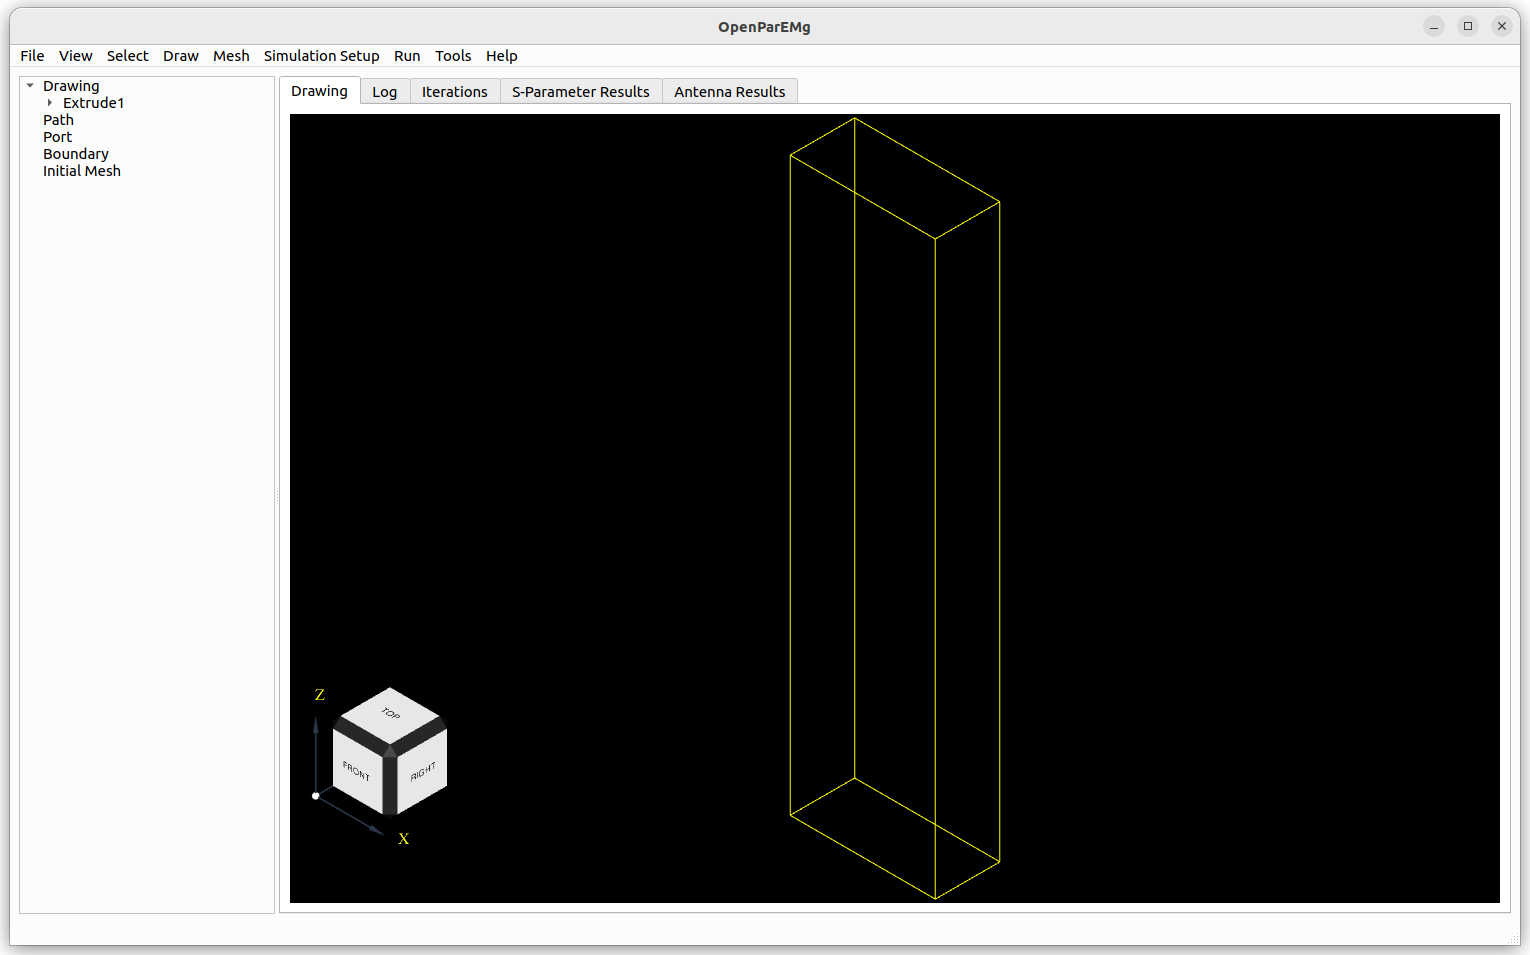
\includegraphics[width=0.75\textwidth]{../tutorials/OpenParEM3D/rectangular_waveguide/OpenParEMg/screenshots/extrusion}
  \caption{Screen shot of the rectangle extruded 90 mm.}
  \label{fig:extrusion}
\end{figure}
\item Click on the rectangular waveguide, then right-click and select \texttt{Edit}.
\item Change the length to $100$ and re-center.
\item Select \texttt{Drawing} in the item tree, right click, and select \texttt{Expand All}.
\item Select \texttt{Rectangle1} and right click.  An edit form appears.
\item Enter 50 for X and click \texttt{Ok}.  The extruded object is recalculated and moved to the new location.  Extrusions can be moved directly and the length can be changed by the edit form, but additional modification is made by editing the underlying 2D object.
\item Re-center the rectangular waveguide.
\item Save the project with \texttt{File}$\rightarrow$\texttt{Save}.

\end{itemize}

\subsubsection{Ports}

\begin{itemize}
\item Select \texttt{Select}$\rightarrow$\texttt{Face}, then select one of the $22.86\times10.16$ rectangles on either end.
\item Right click in the drawing window and click \texttt{Create Port}.  A gray box appears on the selected face and a port item appears in the selection tree along with a matching path.  The default port name is \texttt{port1}, and this can be changed if desired.
\item Expand \texttt{net1} in \texttt{port1} and click on \texttt{voltage}, right click then select \texttt{Draw Line Path}.
\item On the gray area of the new port, click in the center of one long edge then the center of the othe long edge to create an integration path for the voltage.  The characteristic impedance calculation is automatically set to \texttt{PV}.  The new port should look like that in Fig.~\ref{fig:port1}.
\begin{figure}
  \centering
  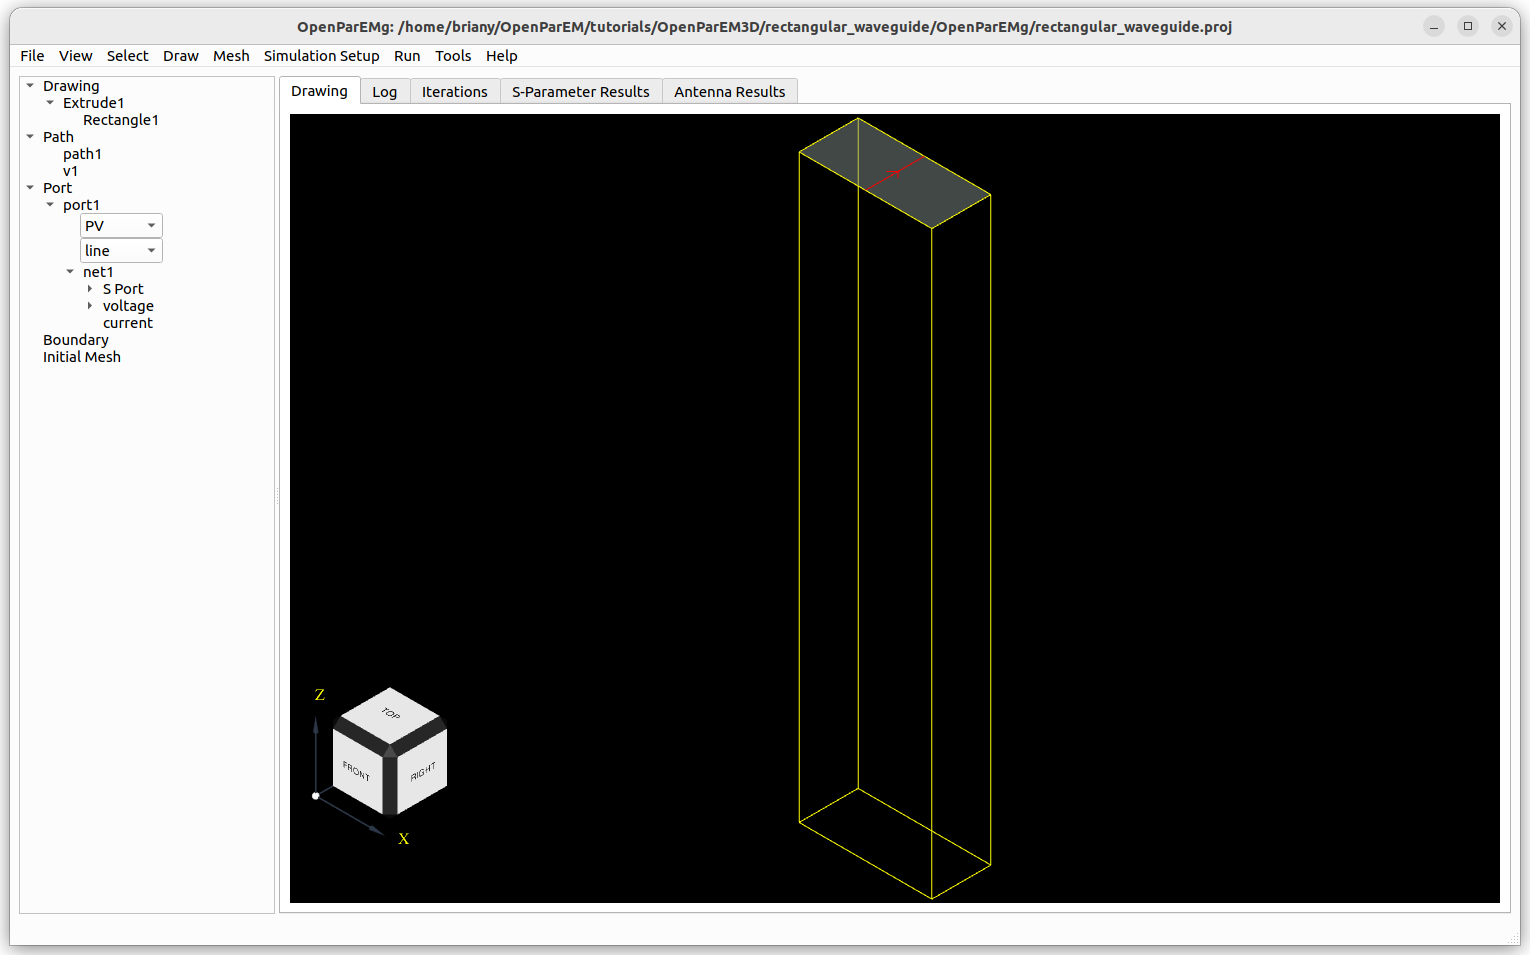
\includegraphics[width=0.75\textwidth]{../tutorials/OpenParEM3D/rectangular_waveguide/OpenParEMg/screenshots/port1}
  \caption{Screen shot of the 100 mm long rectangular waveguide with port 1 added.}
  \label{fig:port1}
\end{figure}
\item Rotate the rectangular waveguide to bring the other end to the front, then repeat the selection of the face and creation of a port along with the drawing of a voltage integration line.  After the creation of the second port, the rectangular waveguide looks like that of Fig.~\ref{fig:ports1and2}.
\begin{figure}
  \centering
  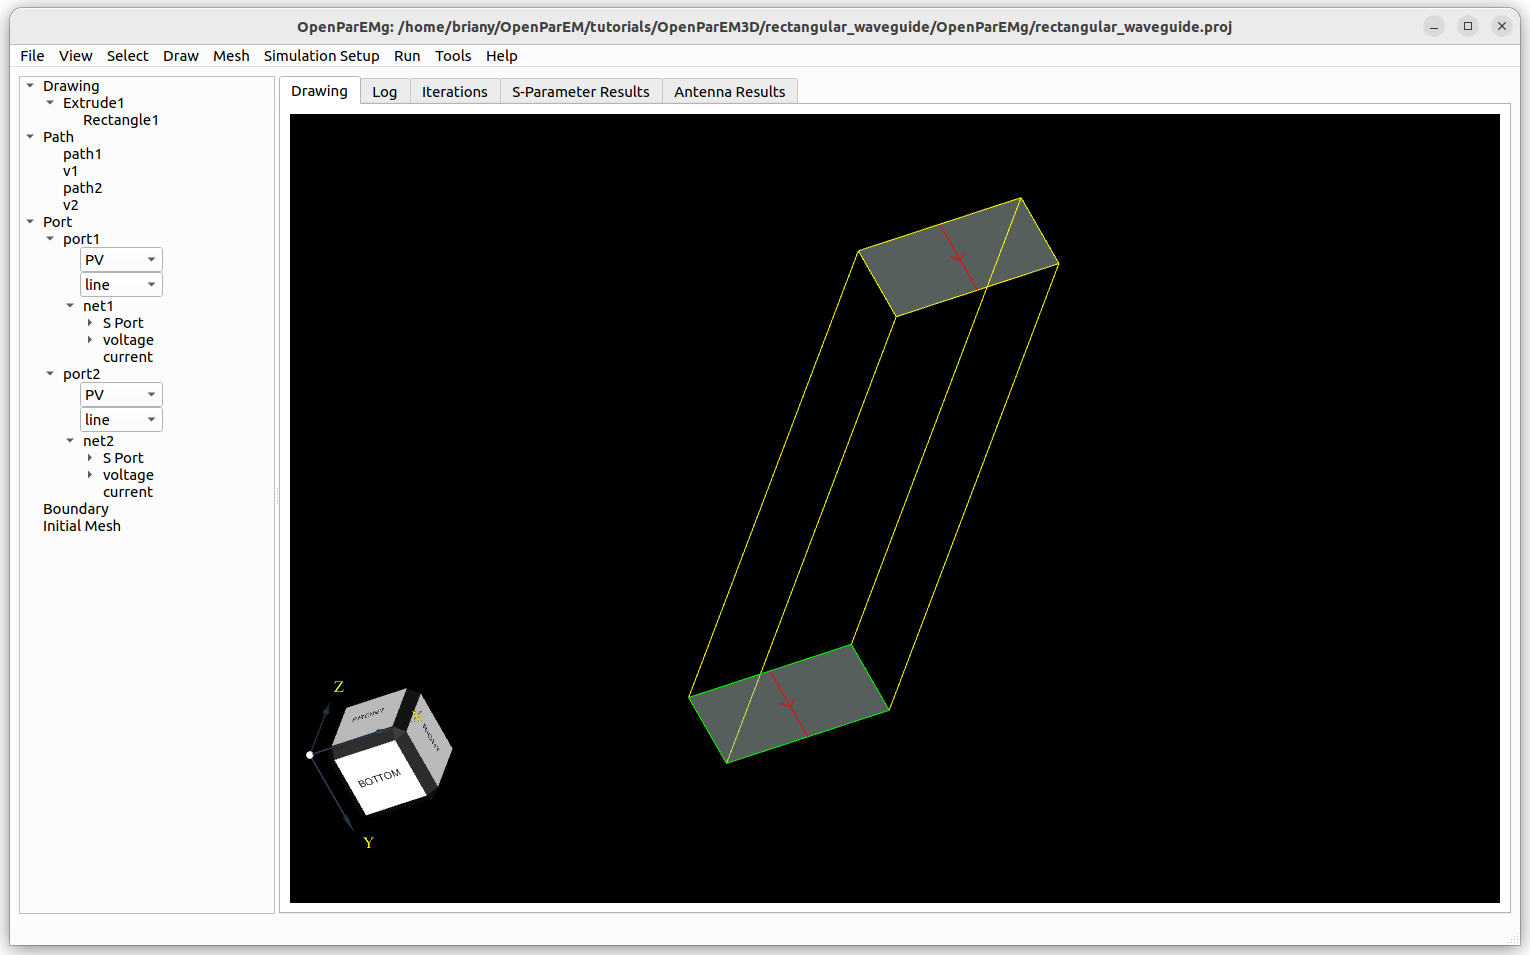
\includegraphics[width=0.75\textwidth]{../tutorials/OpenParEM3D/rectangular_waveguide/OpenParEMg/screenshots/ports1and2}
  \caption{Screen shot of the 100 mm long rectangular waveguide with ports 1 and 2 added.}
  \label{fig:ports1and2}
\end{figure}
\item If the voltage integration paths are not pointing in the same direction, then the computed S-parameters will have a $180$ degree phase shift for S21 and S12.  Direction alignment can be corrected by selecting the path in the drawing window or the selection tree, right clicking, then selecting \texttt{Reverse Direction}.
\item Save the project.
\end{itemize}

\subsubsection{Materials}
\begin{itemize}
\item Create the materials file \texttt{global\_materials.txt} in any text editor and set the text contents to
\begin{Verbatim}[fontsize=\small]
  #OpenParEMmaterials 1.0
  Material
     name=air
     type=dielectric
     Temperature
        temperature=any
        Frequency
           frequency=any
           er=1.0006
           mur=1
           tand=0
           Rz=0
        EndFrequency
     EndTemperature
     Source
        Constantine A. Balanis, "Advanced Engineering Electromagnetics",
        John Wiley and Sons, 1989, p.79.
     EndSource
  EndMaterial
\end{Verbatim}
\item Select \texttt{Simulation Setup}$\rightarrow$\texttt{Materials ...} to bring up a materials selection window.  Click \texttt{global} then right-click, select \texttt{Open ...}, then select the newly created materials file.
\item Select the rectangular waveguide in the drawing window or the item tree, then right click and click \texttt{Assign Material}.  Select \texttt{air} then \texttt{Ok}.
\item Save the project.
\end{itemize}

\subsubsection{Mesh}

\begin{itemize}
\item Select \texttt{Mesh}$\rightarrow$\texttt{Generate}.  The mesh should appear as in Fig.~\ref{fig:mesh}.
\begin{figure}
  \centering
  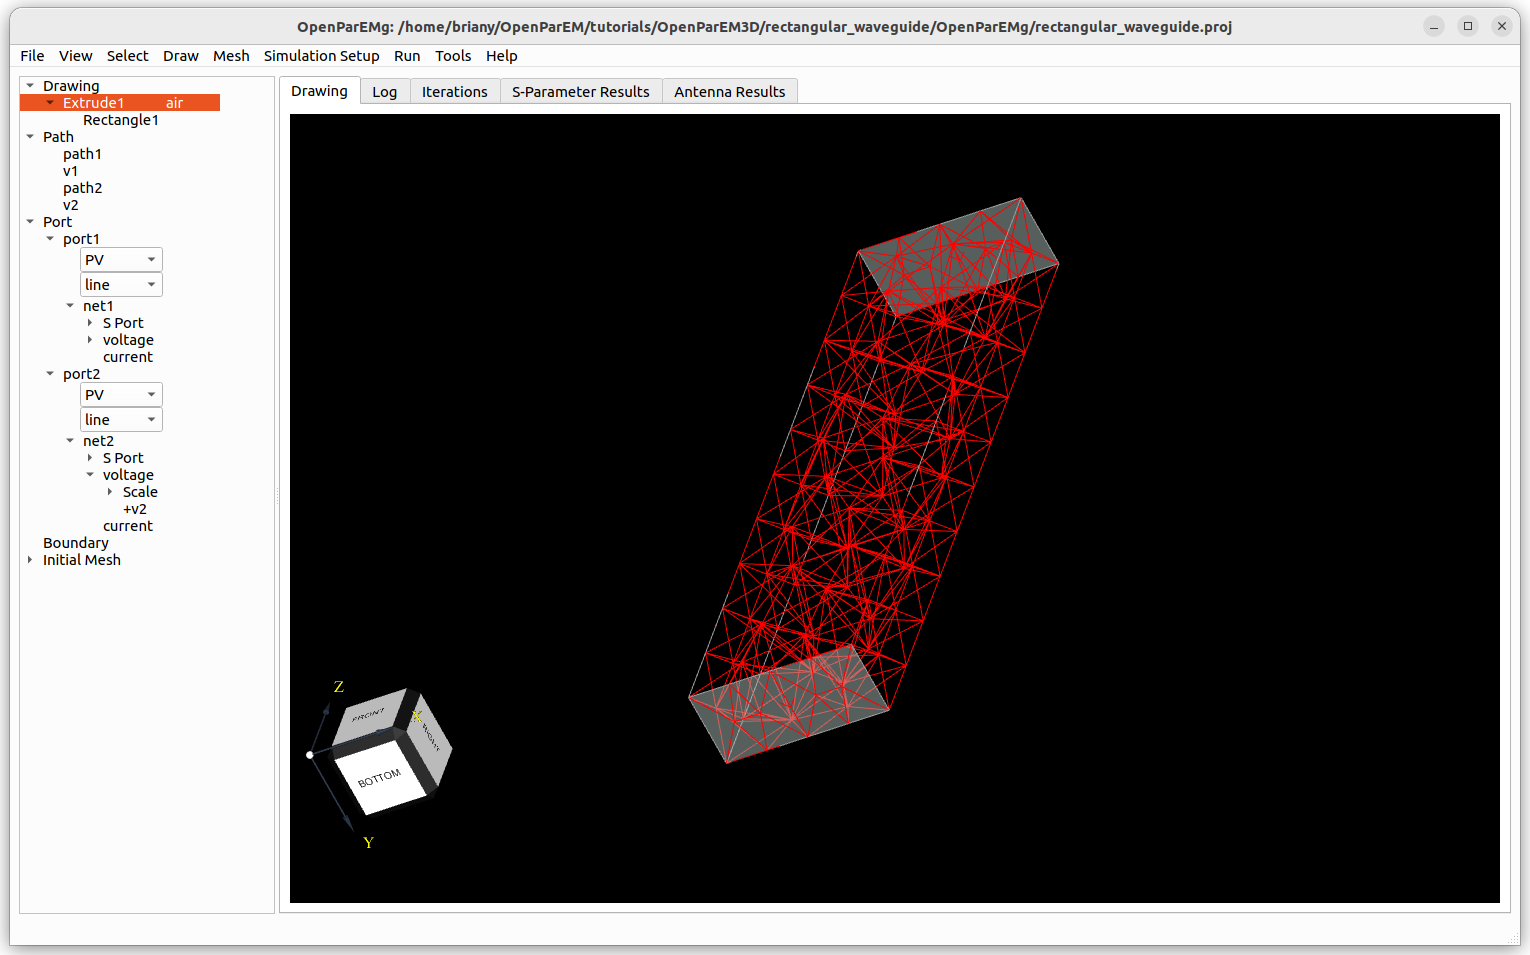
\includegraphics[width=0.75\textwidth]{../tutorials/OpenParEM3D/rectangular_waveguide/OpenParEMg/screenshots/mesh}
  \caption{Meshed rectangular waveguide.}
  \label{fig:mesh}
\end{figure}
\end{itemize}

\subsubsection{Simulation Setup}

\begin{itemize}
\item Select \texttt{Simulation Setup}$\rightarrow$\texttt{Options ...}.
\item On the \texttt{S-Parameters} tab, uncheck \texttt{Normalize}.
\item On the \texttt{Controls} tab, set \texttt{FEM Order} to 4.  Set \texttt{Parallel Processing Slot Count} to a number appropriate for the computer.  See the users manual "OpenParEM3D\_Users\_Manual.pdf" for guidance.  If using MPICH, uncheck \texttt{Oversubscribe}.
\item On the \texttt{Outputs} tab, check \texttt{Save 3D fields}.
\item Click \texttt{Ok}.
\item Select \texttt{Simulation Setup}$\rightarrow$\texttt{Frequency Plan ...}.
\item Uncheck \texttt{AMR}.
\item Click \texttt{Add}.
\item Change the start frequency from $1$ to $10$.
\item Click \texttt{Ok}.
\item Save the project.
\end{itemize}

\subsubsection{Solving}

\begin{itemize}
\item Select \texttt{Run}$\rightarrow$\texttt{Run}.  If the \texttt{Run} option is grayed out, then a step was somehow missed along the way.  Hover over the \texttt{Run}$\rightarrow$\texttt{Run} menu item to get a list of what needs to be done to enable the run to be started.
\item Review the tabs to monitor the job.
\item The simulation results should be very similar to those shown in Fig.~\ref{fig:results}.  Note that the results will not be exactly the same due to the iterative solution in combination with MPI processing.
\begin{figure}
  \centering
  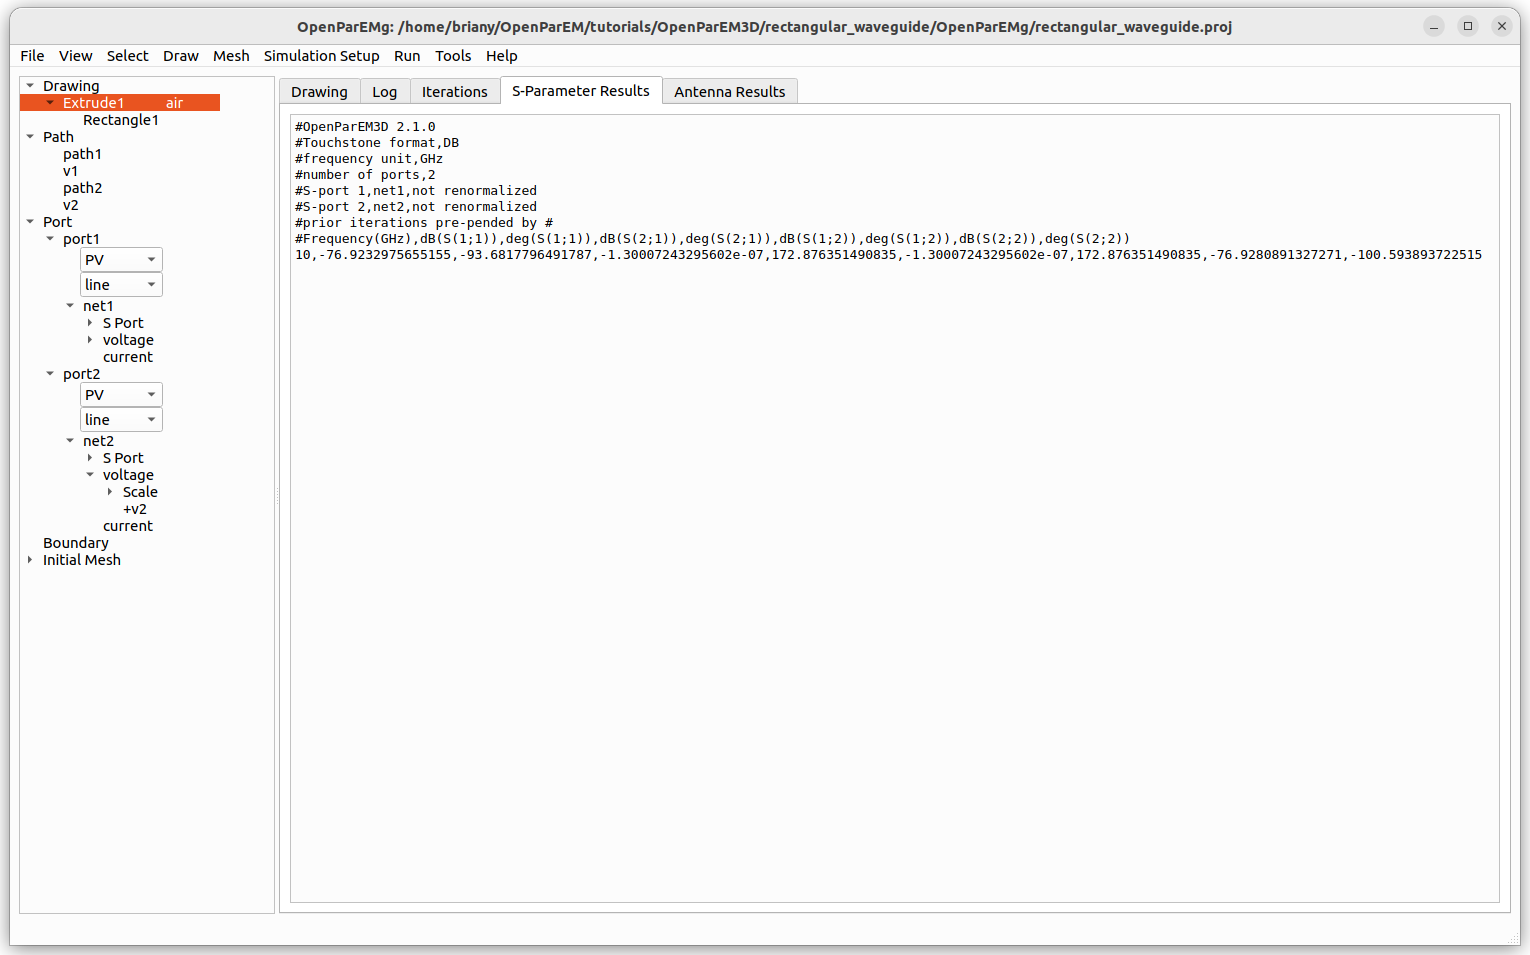
\includegraphics[width=0.75\textwidth]{../tutorials/OpenParEM3D/rectangular_waveguide/OpenParEMg/screenshots/results}
  \caption{Computed results for the rectangular waveguide.}
  \label{fig:results}
\end{figure}
\item From the \texttt{Log} tab, the 2D port simulation shows $\beta=158.32151$~rad/s, so for a 100~mm long waveguide, the total phase shift is $-15.832151$~rad, or $172.88456$~degrees, which well matches the computed S21 phase shift of $172.87635$~degrees.
\item All results are already saved to files, so there is no need for an additional save from OpenParEMg.
\end{itemize}

\subsubsection{3D Plots}

\begin{itemize}
\item OpenParEMg does not support plotting.
\item Start ParaView at the command line with \verb+$ paraview &+, then in the \texttt{Paraview*} directory, navigate to and open the fields result \newline \texttt{rectangular\_waveguide\_frequency\_1e+10\_Sport\_1.pvd}
\item Click in the window and move the mouse to change the view.
\item Click on the box \texttt{Solid Color} then select \texttt{gridReE}.  Click \texttt{Apply} if nothing happens.
\item Click on the box \texttt{Magnitude} and select \texttt{1} to view the y-component of the electric field.  A screen shot is shown in Fig.~\ref{fig:ReEy}.
\begin{figure}[H]
  \centering
  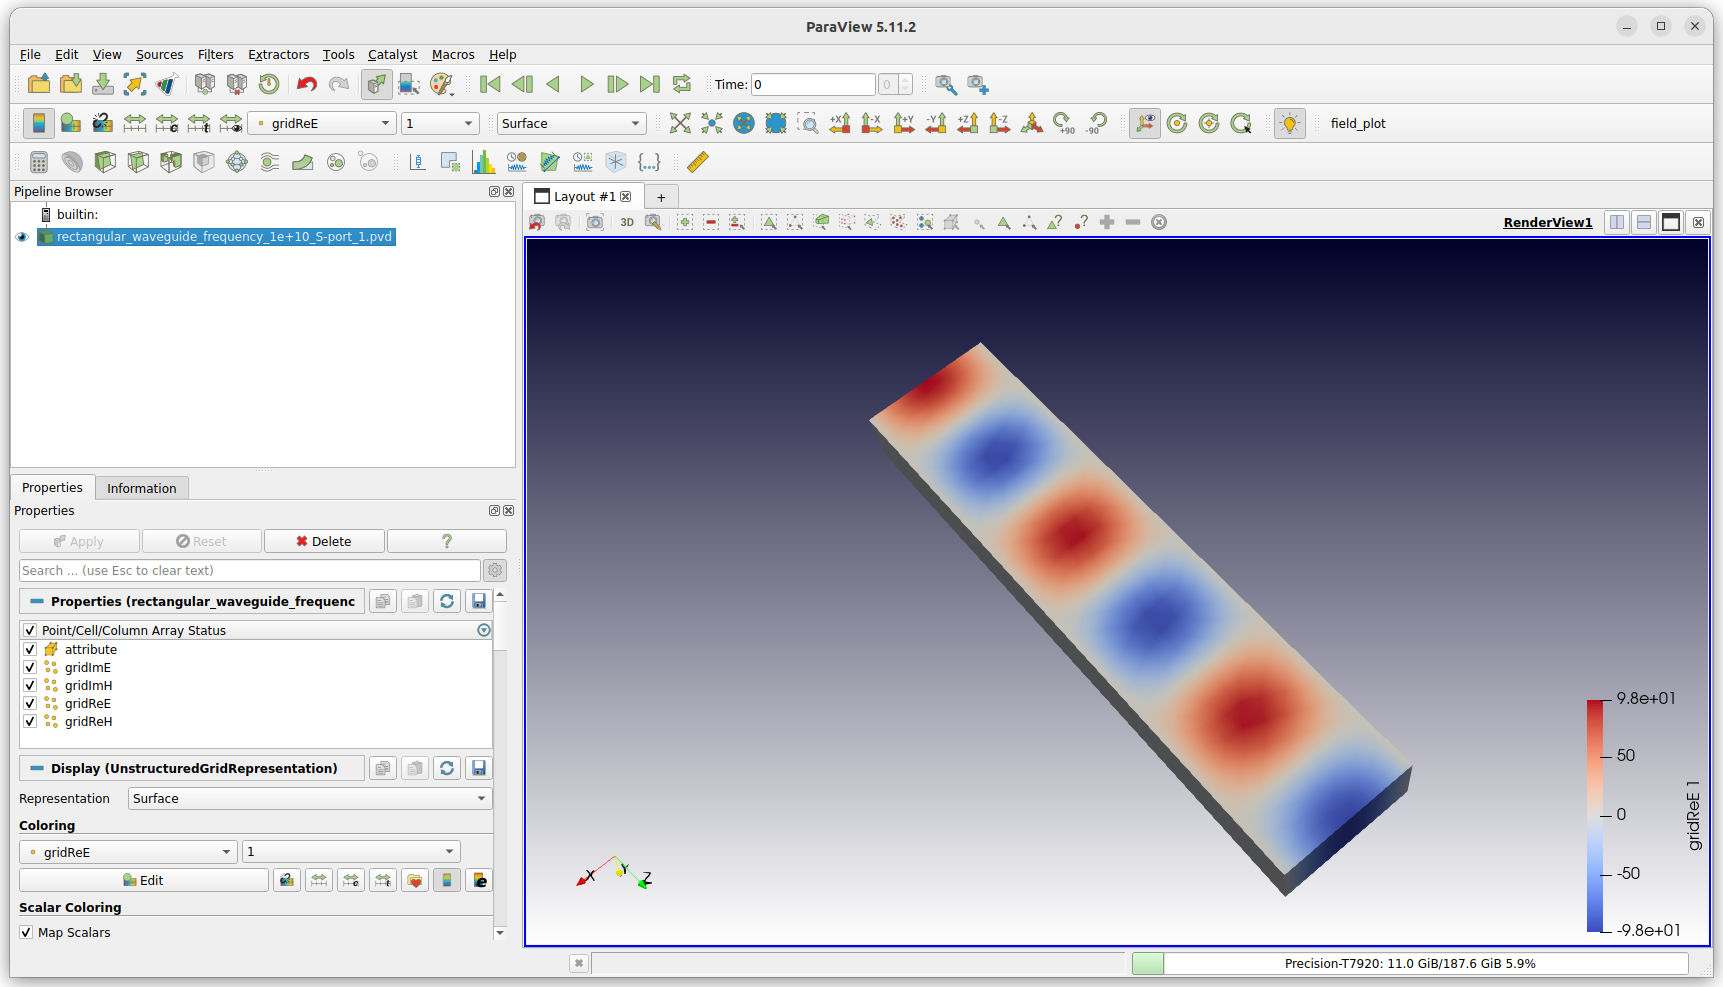
\includegraphics[width=0.75\textwidth]{../tutorials/OpenParEM3D/rectangular_waveguide/OpenParEMg/screenshots/ReEy}
  \caption{Re($E_y$) for the rectangular waveguide when driven by port 1.}
  \label{fig:ReEy}
\end{figure}
\item Vector plots can be viewed by selecting \texttt{Filters}$\rightarrow$\texttt{Alphabetical}$\rightarrow$\texttt{Glyph}.
\item Ensure that the \texttt{Glyph1} item in the \texttt{Pipeline Browser} is selected and that any other items are not.
\item Set \texttt{Orientation Array} to \texttt{gridReE} and the \texttt{Scale Array} to \texttt{gridReE}.
\item Set \texttt{Scale Factor} to 6.3e-05.
\item An outline of the geometry can be created by enabling \texttt{rectangular\_waveguide\_frequency\_1e+10\_Sport\_1.pvd}, then change \texttt{Representation} from \texttt{Surface} to \texttt{Outline}.
\item A similar plot for $\overline{H}$ can also be made.  A scale factor of 0.03 works well.
\item Screenshots for $\overline{E}$ and $\overline{H}$ are shown in Fig.~\ref{fig:fields}.
\begin{figure}[H]
  \centering
  \begin{subfigure}{0.73\textwidth}
     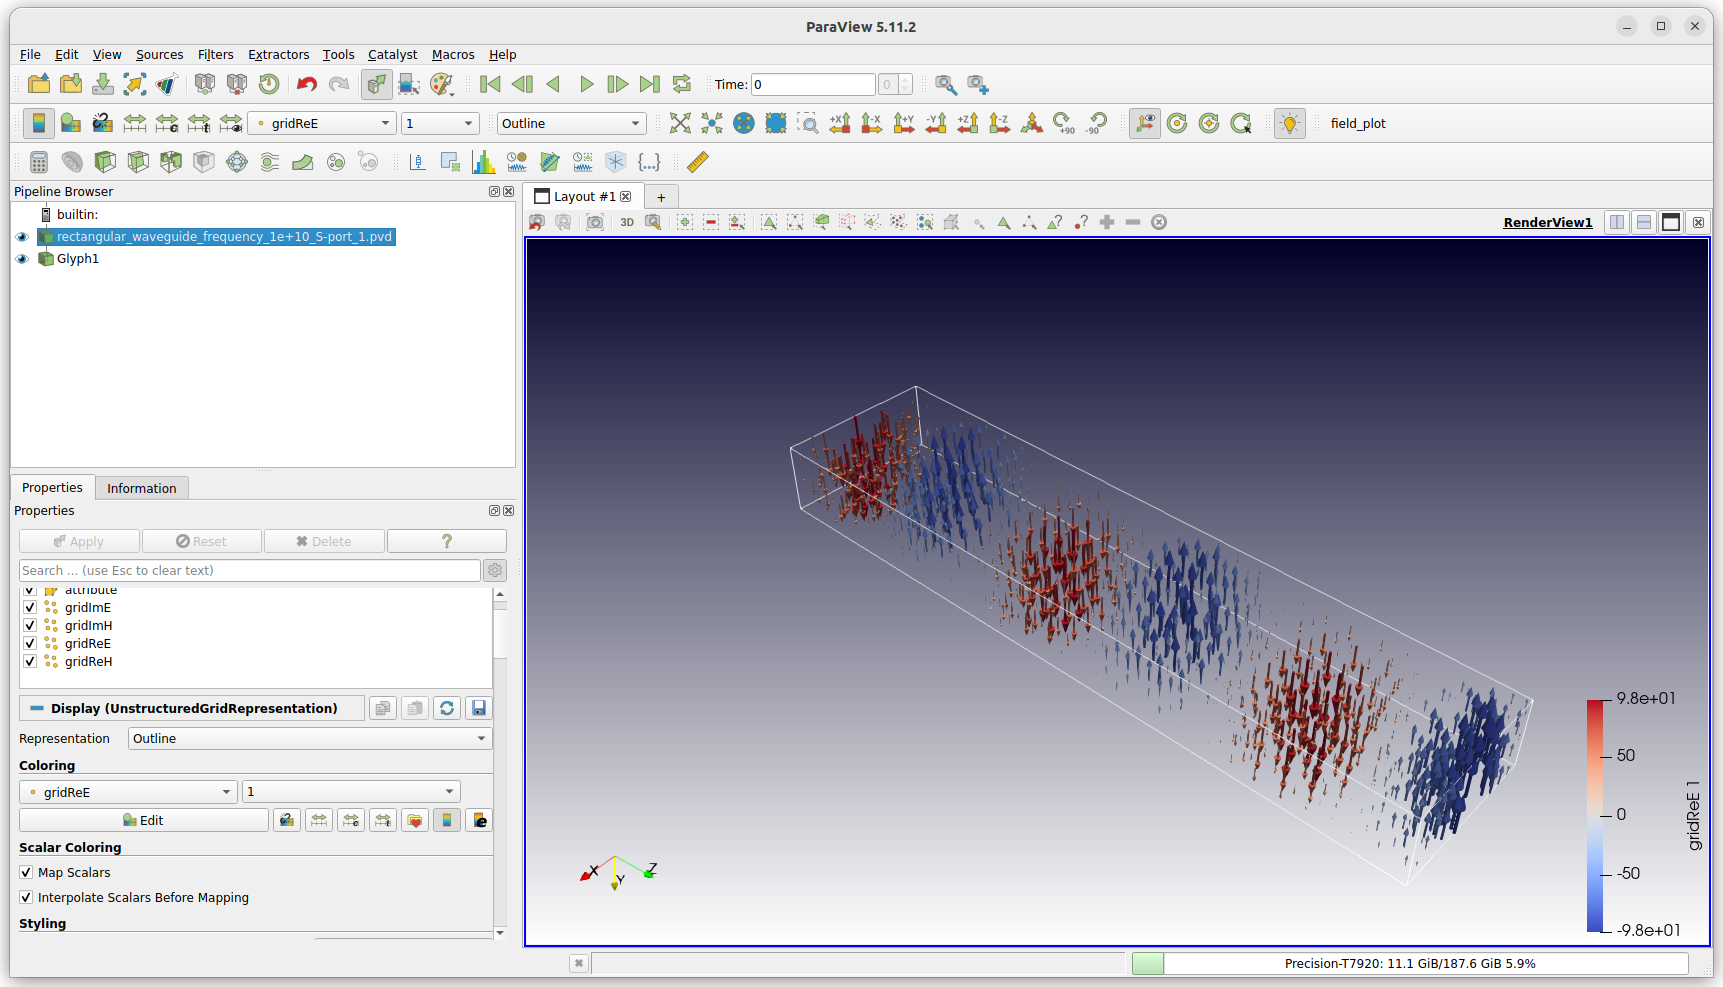
\includegraphics[width=\linewidth]{../tutorials/OpenParEM3D/rectangular_waveguide/OpenParEMg/screenshots/ReE}
     \caption{Re($\overline{E}$)}
  \end{subfigure}
  \par\bigskip
  \begin{subfigure}{0.73\textwidth}
     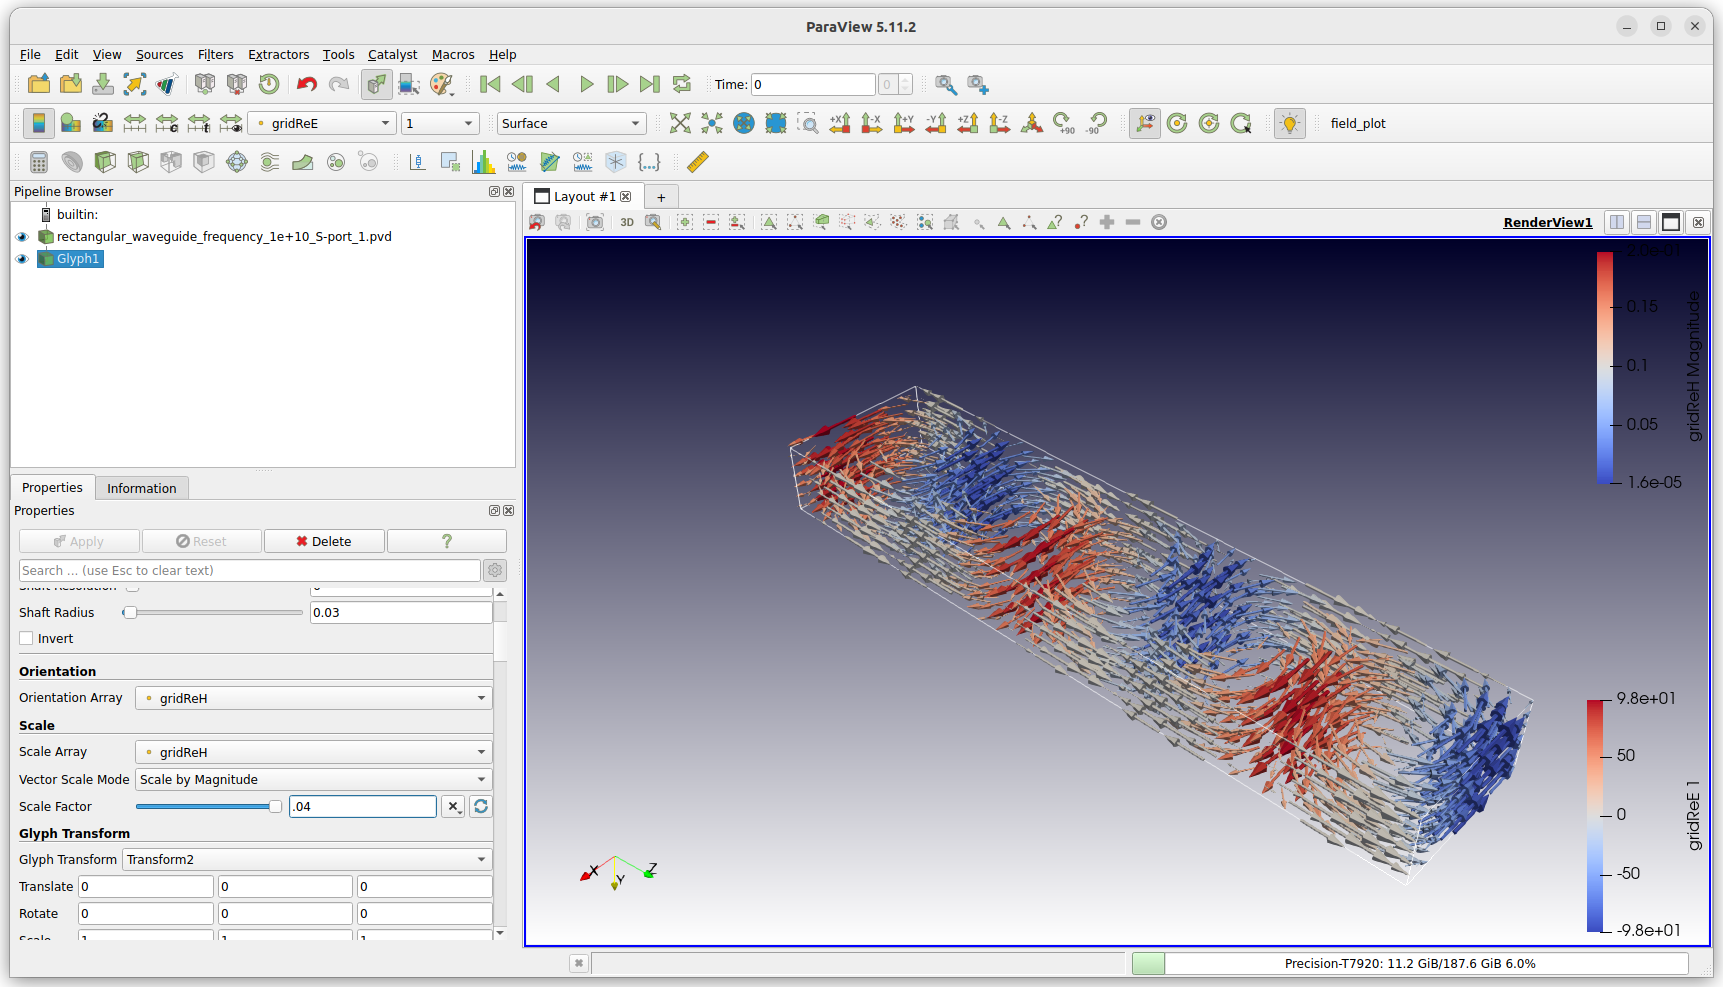
\includegraphics[width=\linewidth]{../tutorials/OpenParEM3D/rectangular_waveguide/OpenParEMg/screenshots/ReH}
     \caption{Re($\overline{H}$)}
  \end{subfigure}
  \caption{Vector fields for the rectangular waveguide when driven by port 1.}
  \label{fig:fields}
\end{figure}

\end{itemize}


\subsection{Microstrip Step in Width}

A straight section of microstrip with a step in width is constructed, annotated for 2-port S-parameter simulation, meshed, and solved.

\subsubsection{Drawing}

\begin{itemize}
\item Create a directory for the project
\begin{Verbatim}[fontsize=\small]
$ mkdir microstrip_step
$ cd microstrip_step
\end{Verbatim}
\item Start OpenParEMg, start a new project with \texttt{File}$\rightarrow$\texttt{New}, then \texttt{File}$\rightarrow$\texttt{Save As ...} to save the project in the new project directory using the name \texttt{microstrip\_step.proj}.
\item For the substrate, draw a rectangle 10~mm long and 2.54~mm wide.  Extrude it 0.254~mm.  Rename the extrusion \texttt{substrate}.
\item For the input microstrip, draw a rectangle 5~mm long and 0.254~mm wide.  Extrude it 0.025~mm.  Rename the extrusion \texttt{input}.
\item Right-click the selected input microstrip, select \texttt{Move}, click the center of the bottom of the end, and then click the center of the top of the substrate.  The drawing should look like that in Fig.~\ref{fig:step_input}.
\begin{figure}[H]
  \centering
  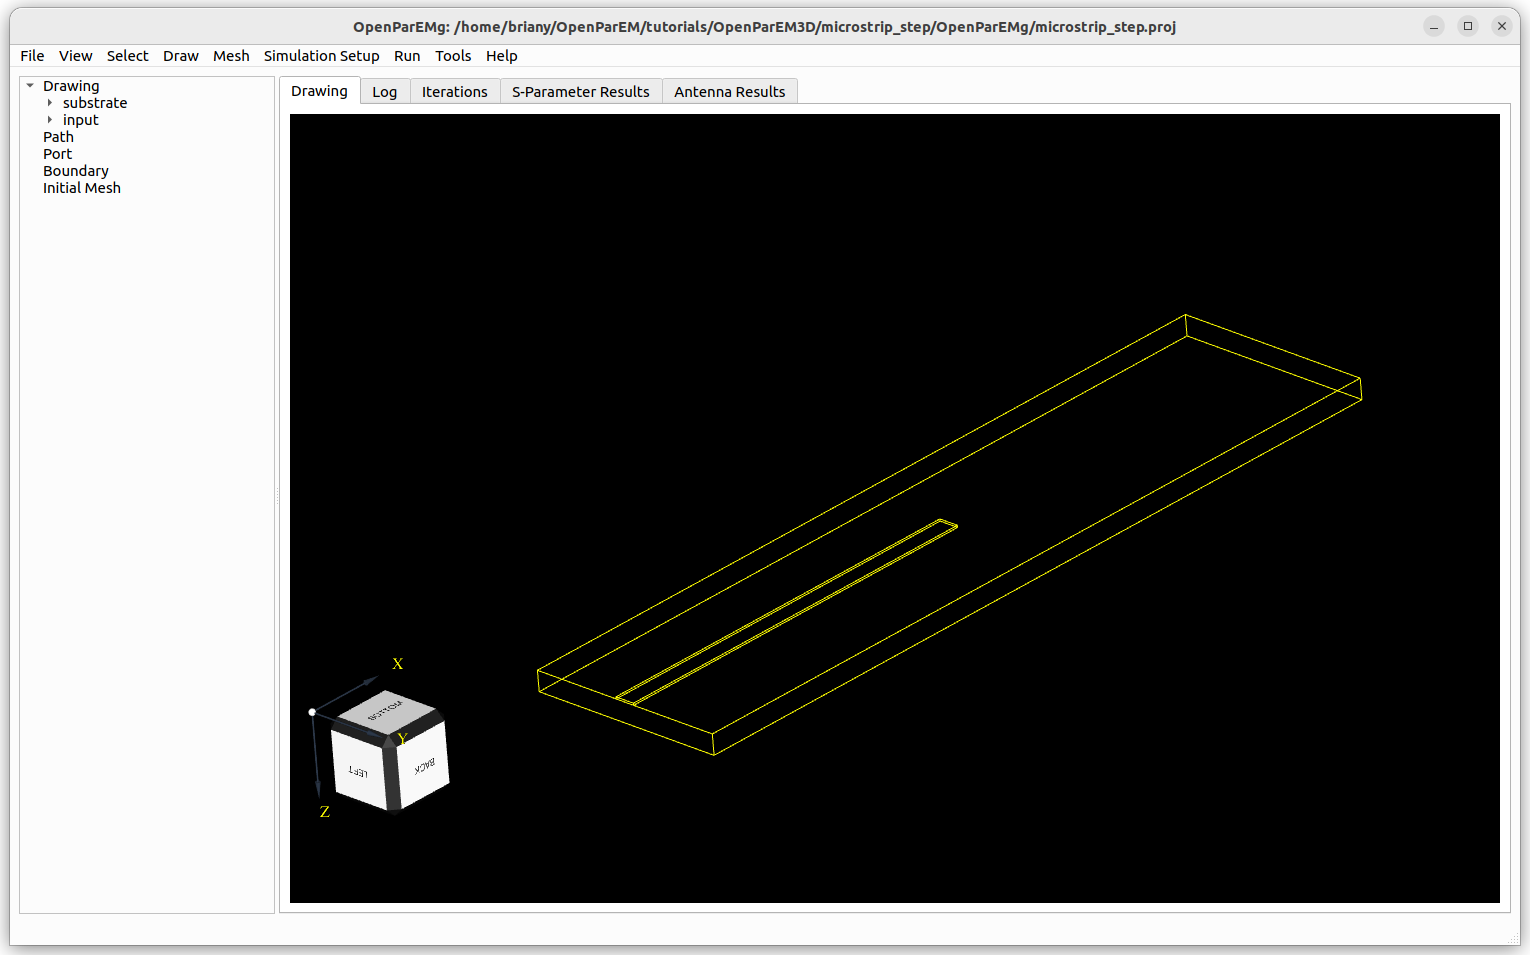
\includegraphics[width=0.75\textwidth]{../tutorials/OpenParEM3D/microstrip_step/OpenParEMg/screenshots/step_input}
  \caption{Substrate and input microstrip.}
  \label{fig:step_input}
\end{figure}
\item For the output microstrip, draw a rectangle 5~mm long and 0.508~mm wide.  Extrude it 0.025~mm, and rename it \texttt{output}.
\item Select and move the output microstrip to align the center of the near end to the center of the far end of the input microstrip.
\item For the air over the microstrip step, expand \texttt{substrate} and select \texttt{Rectangle1}.  Right-click and click \texttt{Copy}.  A new rectange called \texttt{Rectange1\_copy} appears in the selection tree.
\item Select the new rectangle if not already selected, and move it to the top of the substrate.
\item Extrude the new rectangle 1.27~mm and rename it \texttt{air}.
\item The drawing should now look like that in Fig.~\ref{fig:step_pieces}.
\begin{figure}[H]
  \centering
  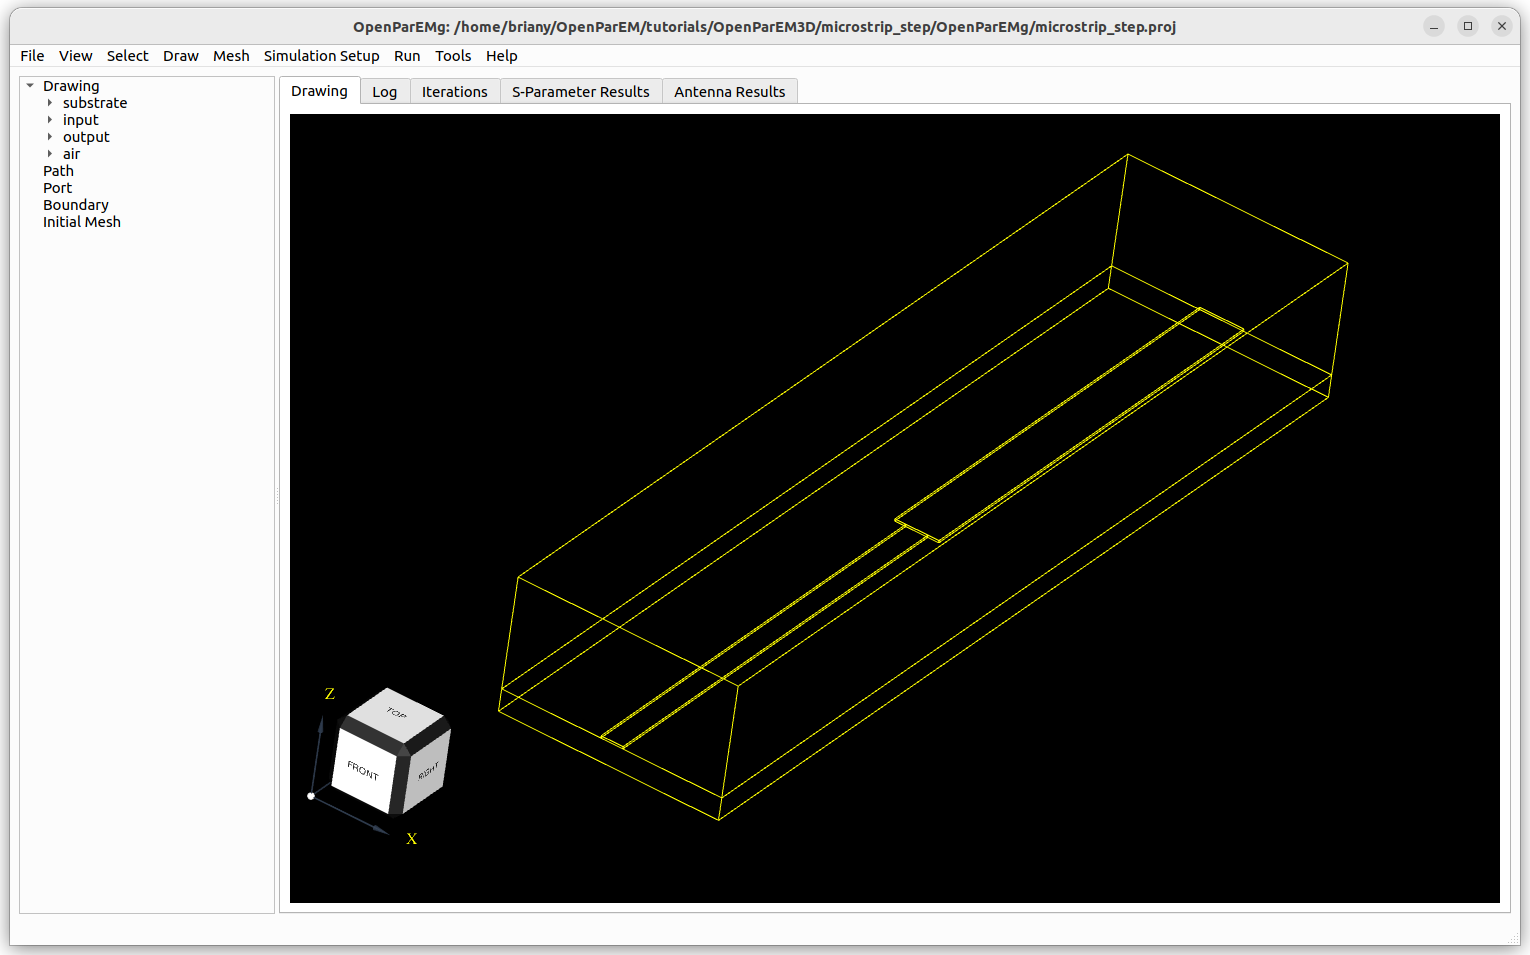
\includegraphics[width=0.75\textwidth]{../tutorials/OpenParEM3D/microstrip_step/OpenParEMg/screenshots/step_pieces}
  \caption{Substrate, input and output microstrips, and air.}
  \label{fig:step_pieces}
\end{figure}
\item The input and output microstrips must be subtracted from the air, making the microstrip line a void.  Voids have the default boundary condition of perfect electric conductor (PEC), making the microstrip a conductor.  The air and substrate volumes are dielectrics.
\item Select \texttt{input} and \texttt{output}, right click, and click \texttt{Merge}.  Rename the merged item as \texttt{step}.
\item Select \texttt{air} and \texttt{step}, right click, and click \texttt{Subtract}.  Rename the subtracted item as \texttt{air-metal}.  The order is important for subtraction operations since the second selected item is subtracted from the first.
\item Save the project.
\end{itemize}

\subsubsection{Ports}

\begin{itemize}
\item Orient the drawing so that the input microstrip is towards the front.
\item Select \texttt{Draw}$\rightarrow$\texttt{Drawing Plane ...}$\rightarrow$\texttt{Set to Face}, then click on a face of either \texttt{air} or \texttt{substrate} next to the end of the microstrip input line.
\item Draw a rectangle that covers both the air and substrate faces.  Be sure to snap to the two corners of the structure.
\item Select the new rectangle if not already selected, then right click and click \texttt{Convert to Port}.  A gray box should now cover the end of the 3D structure.
\item Draw a construction box from the substrate corner to the center of the bottom of the input traces.
\item Add a voltage integration line between the bottom of the substrate to the top of the substrate, which is also the bottom of the microstrip line.  Use the construction rectangle as a guide.  The constructed port~1 should look like that in Fig.~\ref{fig:step_port1}.
\begin{figure}[H] 
  \centering
  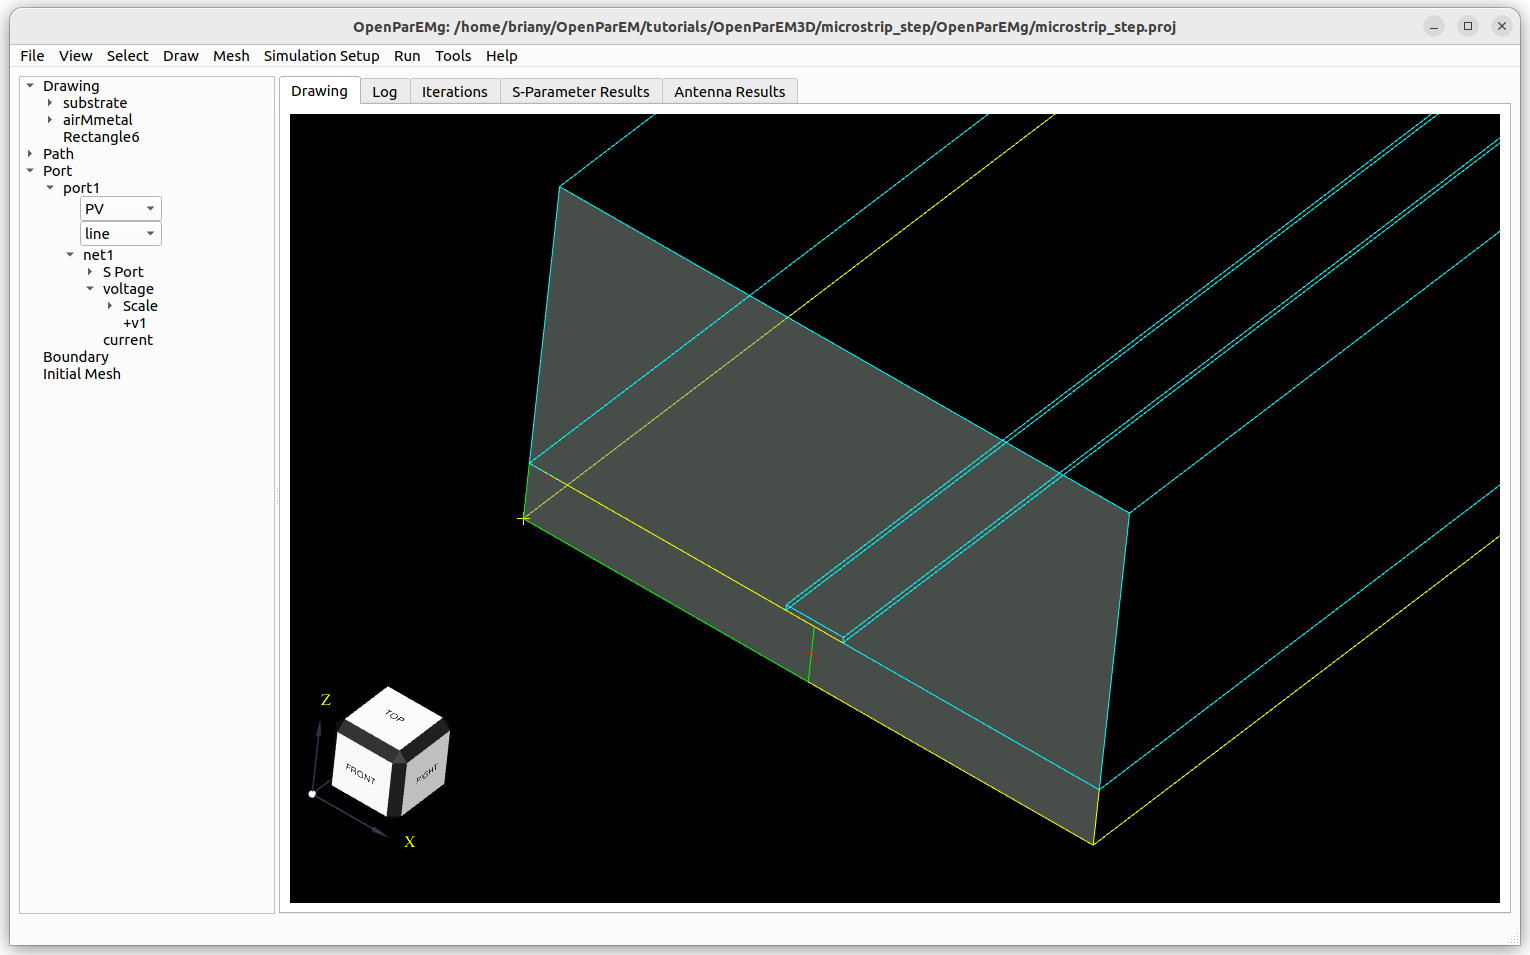
\includegraphics[width=0.75\textwidth]{../tutorials/OpenParEM3D/microstrip_step/OpenParEMg/screenshots/step_port1}
  \caption{Port 1 view with construction rectange shown in green and integration path with red arrowhead.}
  \label{fig:step_port1}
\end{figure}
\item Delete the construction rectangle by highlighting it, right clicking, and clicking \texttt{Delete}.  The full integegration path becomes visible.
\item Repeat the process on the other end for port~2, starting with setting the drawing plane to a face on port~2.  The completed port setup should like that that in Fig.~\ref{fig:step_ports1and2}.
\begin{figure}[H]
  \centering
  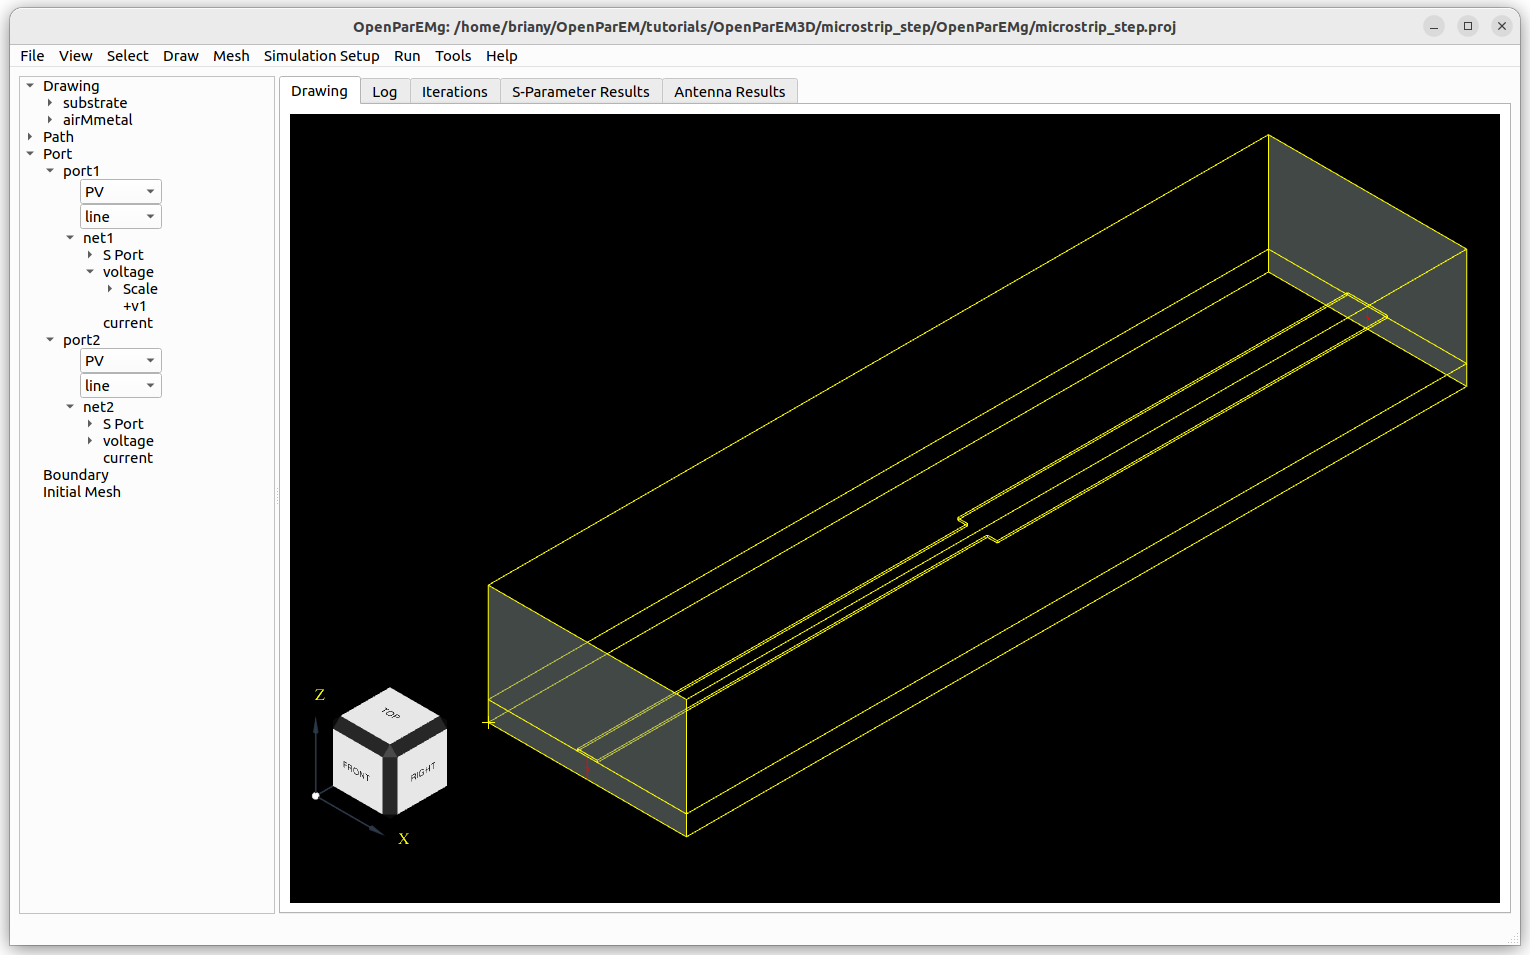
\includegraphics[width=0.75\textwidth]{../tutorials/OpenParEM3D/microstrip_step/OpenParEMg/screenshots/step_ports1and2}
  \caption{Completed port setup for the microstrip step.}
  \label{fig:step_ports1and2}
\end{figure}
\item Save the project.
\end{itemize}

\subsubsection{Materials}

\begin{itemize}
\item Create the materials file \texttt{local\_materials.txt} in any text editor and set the text contents to
\begin{Verbatim}[fontsize=\small]
#OpenParEMmaterials 1.0
Material
   name=air
   type=dielectric
   Temperature
      temperature=any
      Frequency
         frequency=any
         er=1.0006
         mur=1
         tand=0
         Rz=0
      EndFrequency
   EndTemperature
   Source
      Constantine A. Balanis, "Advanced Engineering Electromagnetics",
      John Wiley and Sons, 1989, p.79.
   EndSource
EndMaterial

Material
   name=alumina
   Temperature
      temperature=any
      Frequency
         frequency=any
         er=9.8
         mur=1
         tand=0.001
         Rz=0
      EndFrequency
   EndTemperature
   Source
      Generic numbers for testing.
   EndSource
EndMaterial
\end{Verbatim}

\item Select \texttt{Simulation Setup}$\rightarrow$\texttt{Materials ...} to bring up a materials selection window.  Click \texttt{local} then right-click, select \texttt{Open ...}, then select the newly created materials file.
\item Select \texttt{substrate} in the drawing window or the item tree, then right click and click \texttt{Assign Material}.  Select \texttt{alumina} then \texttt{Ok}.  Select \texttt{air-metal} and assign its material to \texttt{air}.
\item Save the project.
\end{itemize}

\subsubsection{Mesh}

\begin{itemize}
\item Select \texttt{Mesh}$\rightarrow$\texttt{Generate}.  The mesh should appear as in Fig.~\ref{fig:step_mesh}.
\begin{figure}
  \centering
  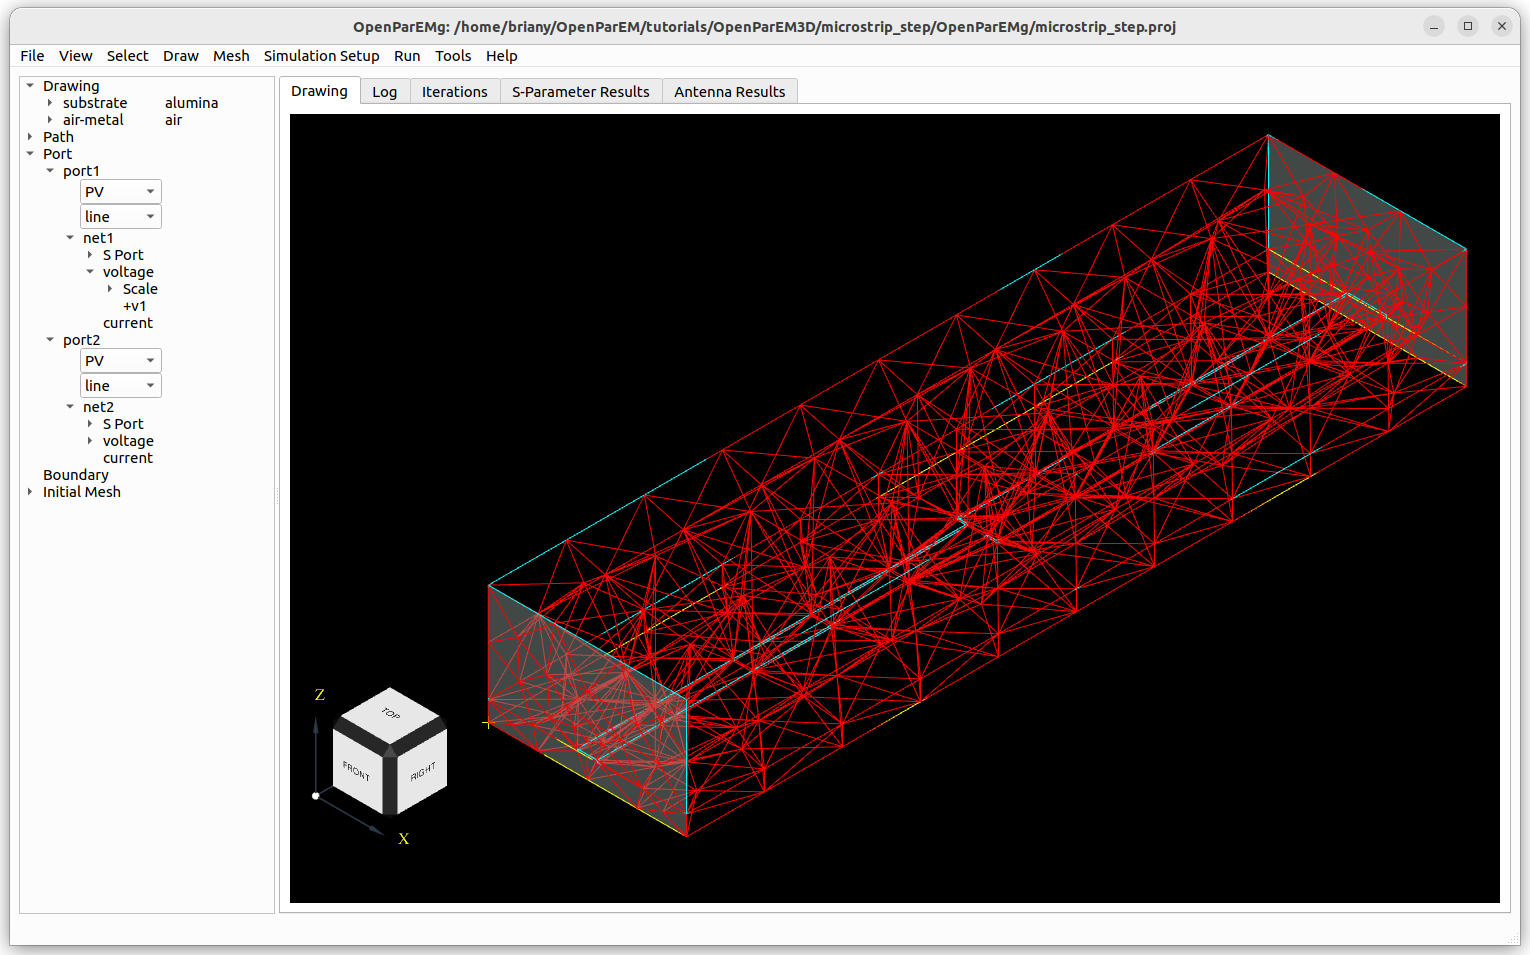
\includegraphics[width=0.75\textwidth]{../tutorials/OpenParEM3D/microstrip_step/OpenParEMg/screenshots/step_mesh}
  \caption{Meshed microstrip step.}
  \label{fig:step_mesh}
\end{figure}
\item Select \texttt{Mesh}$\rightarrow$\texttt{Options ...} and change the \texttt{Refinement Fraction} to $0.001$ to help concentrate adaptive mesh refinement on the edges.  Change the \texttt{Quality Limit} to $100000$. Click \texttt{Ok}.
\end{itemize}

\subsubsection{Simulation Setup}

\begin{itemize}
\item Select \texttt{Simulation Setup}$\rightarrow$\texttt{Options ...}.
\item On the \texttt{S-Parameters} tab, uncheck \texttt{Normalize}.
\item On the \texttt{Controls} tab, set \texttt{FEM Order} to 3.  Set \texttt{Parallel Processing Slot Count} to a number appropriate for the computer.  See the users manual "OpenParEM3D\_Users\_Manual.pdf" for guidance.  If using MPICH, uncheck \texttt{Oversubscribe}.
\item On the \texttt{Outputs} tab, check \texttt{Save 3D fields}.
\item Click \texttt{Ok}.
\item Select \texttt{Simulation Setup}$\rightarrow$\texttt{Frequency Plan ...}.
\item Click \texttt{Add}.
\item Change the start frequency from $1$ to $10$.
\item Click \texttt{Ok}.
\item Select \texttt{Simulation Setup}$\rightarrow$\texttt{Refinement ...}.
\item Set \texttt{Minimum} to $3$.  Set \texttt{Maximum} to $40$.
\item Set \texttt{Refinement Varible} to \texttt{S}.  Set \texttt{Relative S} to $0.01$.
\item Click \texttt{Ok}.
\item Save the project.
\end{itemize}

\subsubsection{Solving}

\begin{itemize}
\item Select \texttt{Run}$\rightarrow$\texttt{Run}.  If the \texttt{Run} option is grayed out, then a step was somehow missed along the way.  Hover over the \texttt{Run}$\rightarrow$\texttt{Run} menu item to get a list of what needs to be done to enable the run to be started.
\item Review the tabs to monitor the job.
\item The simulation results should be very similar to those shown in Fig.~\ref{fig:step_results}.  Note that the results will not be exactly the same due to the iterative solution in combination with MPI processing.
\begin{figure}
  \centering
  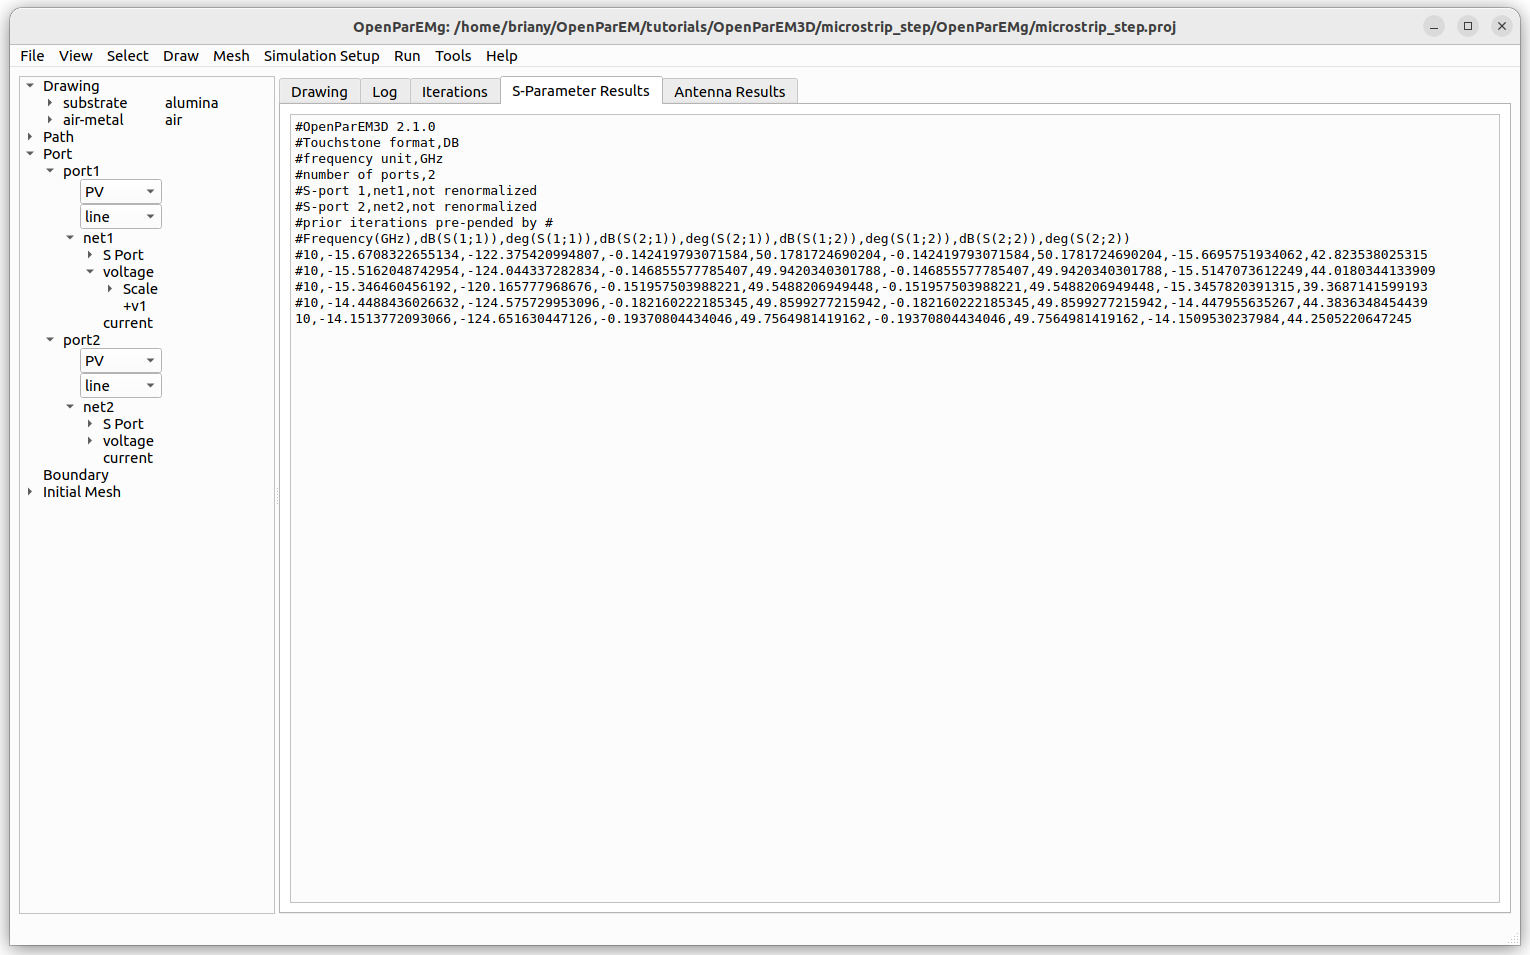
\includegraphics[width=0.75\textwidth]{../tutorials/OpenParEM3D/microstrip_step/OpenParEMg/screenshots/step_results}
  \caption{Computed results for the microstrip step.}
  \label{fig:step_results}
\end{figure}
\item The log tab shows the results from the 2D port simulations, and the impedances for the input and output ports are 46.79~$\Omega$ and 32.77~$\Omega$, respectively.  Considering just the transmission lines, the return loss from these impedances is 20*log10(abs(32.77-46.79)/(32.77+46.79))=-15.09~dB, which is close to the computed value of -14.15~dB.  Note also the expected close values for \textbar S11\textbar and \textbar S22\textbar.
\item All results are already saved to files, so there is no need for an additional save from OpenParEMg.
\end{itemize}

\subsubsection{3D Plots}

\begin{itemize}
\item OpenParEMg does not support plotting.
\item Start ParaView and open the results file for port 1.
\item Add a filter by selecting \texttt{Filters}$\rightarrow$\texttt{Alphabetical}$\rightarrow$\texttt{Slice}.
\item In \texttt{Plane Parameters} select \texttt{Z Normal}, uncheck \texttt{Show Plane}, and change the z-component of the origin to 0.0002.
\item Click the \texttt{-Z} axis orientation on the tool bar.
\item Change \texttt{Solid Color} to \texttt{gridReE} and change the value shown from \texttt{Magnitude} to \texttt{Z} or \texttt{2}, depending on the version of ParaView.  In the buttons below, change the scale to be symmetric with a range of -4000 to +4000.
\item A screen shot of the resulting Re($E_z$) field just under the microstrip traces is shown in Fig.~\ref{fig:step_ReEz}.
\begin{figure}[H]
  \centering
  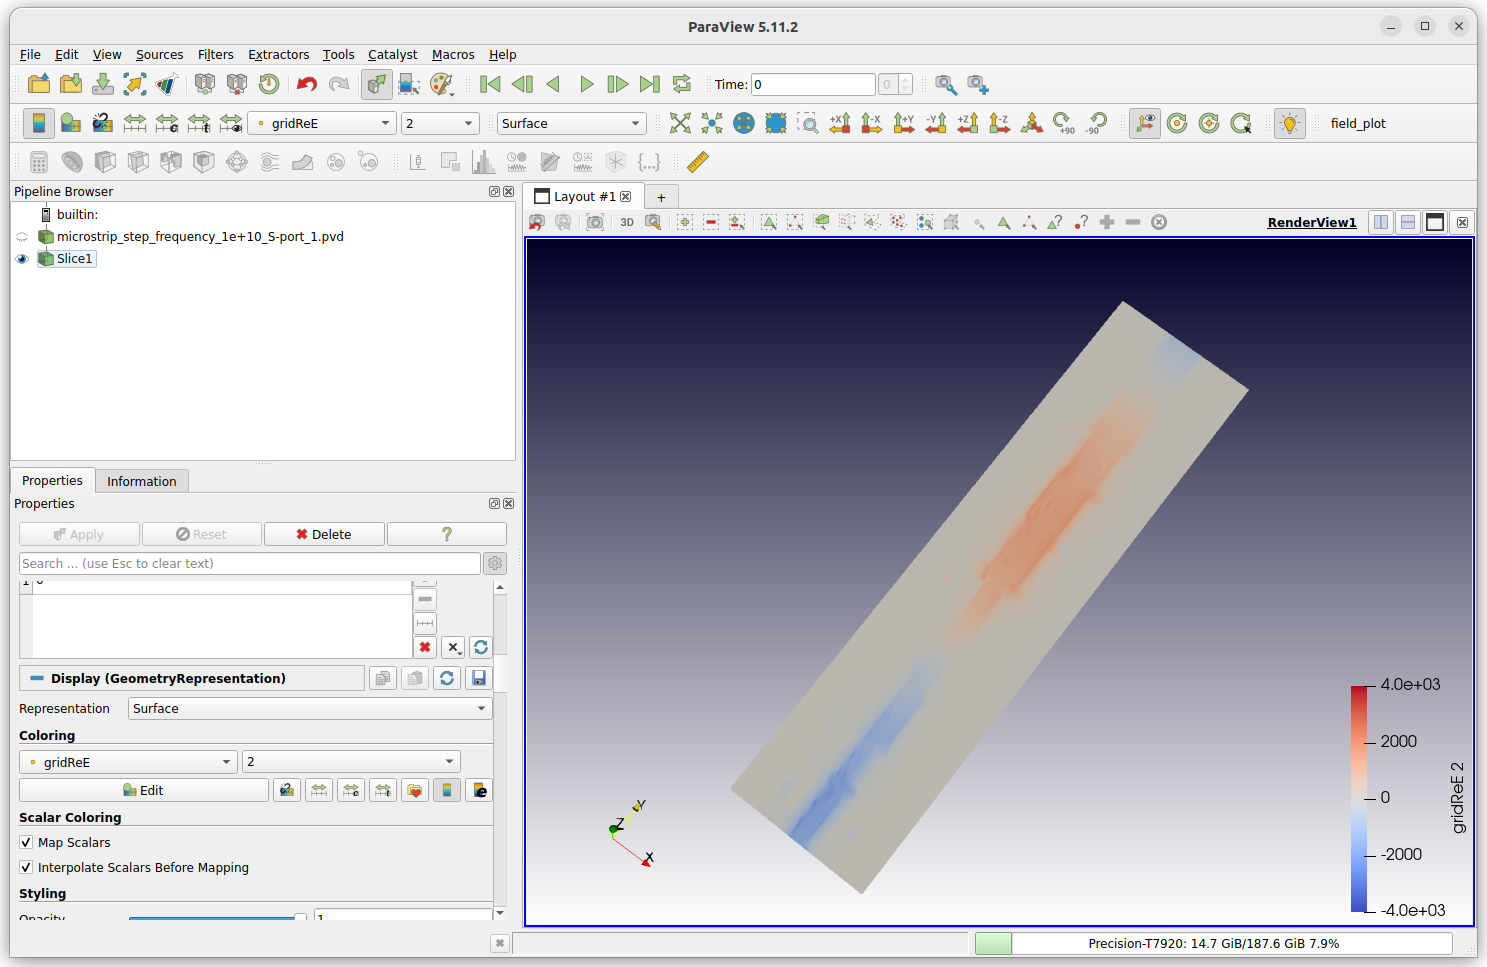
\includegraphics[width=0.75\textwidth]{../tutorials/OpenParEM3D/microstrip_step/OpenParEMg/screenshots/step_ReEz}
  \caption{Screenshot of Re($E_z$) just under the microstrip lines.}
  \label{fig:step_ReEz}
\end{figure}
\end{itemize}

\subsection{Monopole Antenna}
\label{sec:monpoleantenna}

A monopole antenna with coax feed is constructed and annotated for 1-port S-parameter simulation, meshed, and solved.

\subsubsection{Drawing}

\begin{itemize}
\item Create a directory for the project
\begin{Verbatim}[fontsize=\small]
$ mkdir monopole_antenna
$ cd monopole_antenna
\end{Verbatim}
\item Start OpenParEMg, start a new project with \texttt{File}$\rightarrow$\texttt{New}, then \texttt{File}$\rightarrow$\texttt{Save As ...} to save the project in the new project directory using the name \texttt{monopole\_antenna.proj}.
\item The first drawing task is to draw the coaxial feed.
\item For the center conductor of the coax, select \texttt{Draw}$\rightarrow$\texttt{polycircle} and draw a circle of any size.
\item Right click and click \texttt{Edit}.
\item Set the center position X and Y to 0, and in the boxes after the \texttt{OR}, set X=0.6 and Y=0. The radius should then show as 0.6.
\item Extrude the new polycircle 2~mm.  Rename it \texttt{pin}.
\item For the coax dielectric, select and copy \texttt{pin} and rename it \texttt{dielectric}.  Expand \texttt{dielectric}, select the polycircle, and edit it to change the radius to 2.07~mm.  The extrusion will re-calculate.
\item Copy \texttt{dielectric} and rename it \texttt{body}.  Edit its polycircle and change the radius to 2.5~mm.
\item Edit \texttt{body} and change the extrusion length to 3~mm.  It now sticks up 1~mm, so it needs to be moved down 1~mm.
\item Expand \texttt{body} and edit the polycircle.  Change the center position Z to -1 and clieck \texttt{Ok}.  The extrusion will re-calculate.
\item Make the pin a conductor by subtracting it from the dielectric, so select \texttt{dielectric} and CTRL-select \texttt{pin}, then right click and select \texttt{Subtract}.  Rename this \texttt{coax}.
\item The next drawing task is to draw the ground plane.
\item Draw a rectangle of any size, then edit it to set the position to X=-50, Y=-50, Z=2, and width=100 and height=100. Extrude it by -0.5~mm amd remame the extrusion \texttt{gp}. Note the minus sign on the extrusion direction.
\item The next item is the monopole.
\item Draw a polycircle of any size.
\item Edit the polycircle and set the position to X=0, Y=0, Z=2, and in the \texttt{OR} area, set X=1, Y=0.  The radius should recalculate to 1~mm.  Extrude the new polycircle by 15~mm, and rename it \texttt{monopole}.
\item A zoom of the coax and monopole antenna should look like that of Fig.~\ref{fig:monopole_zoom}.
\begin{figure}[H]
  \centering
  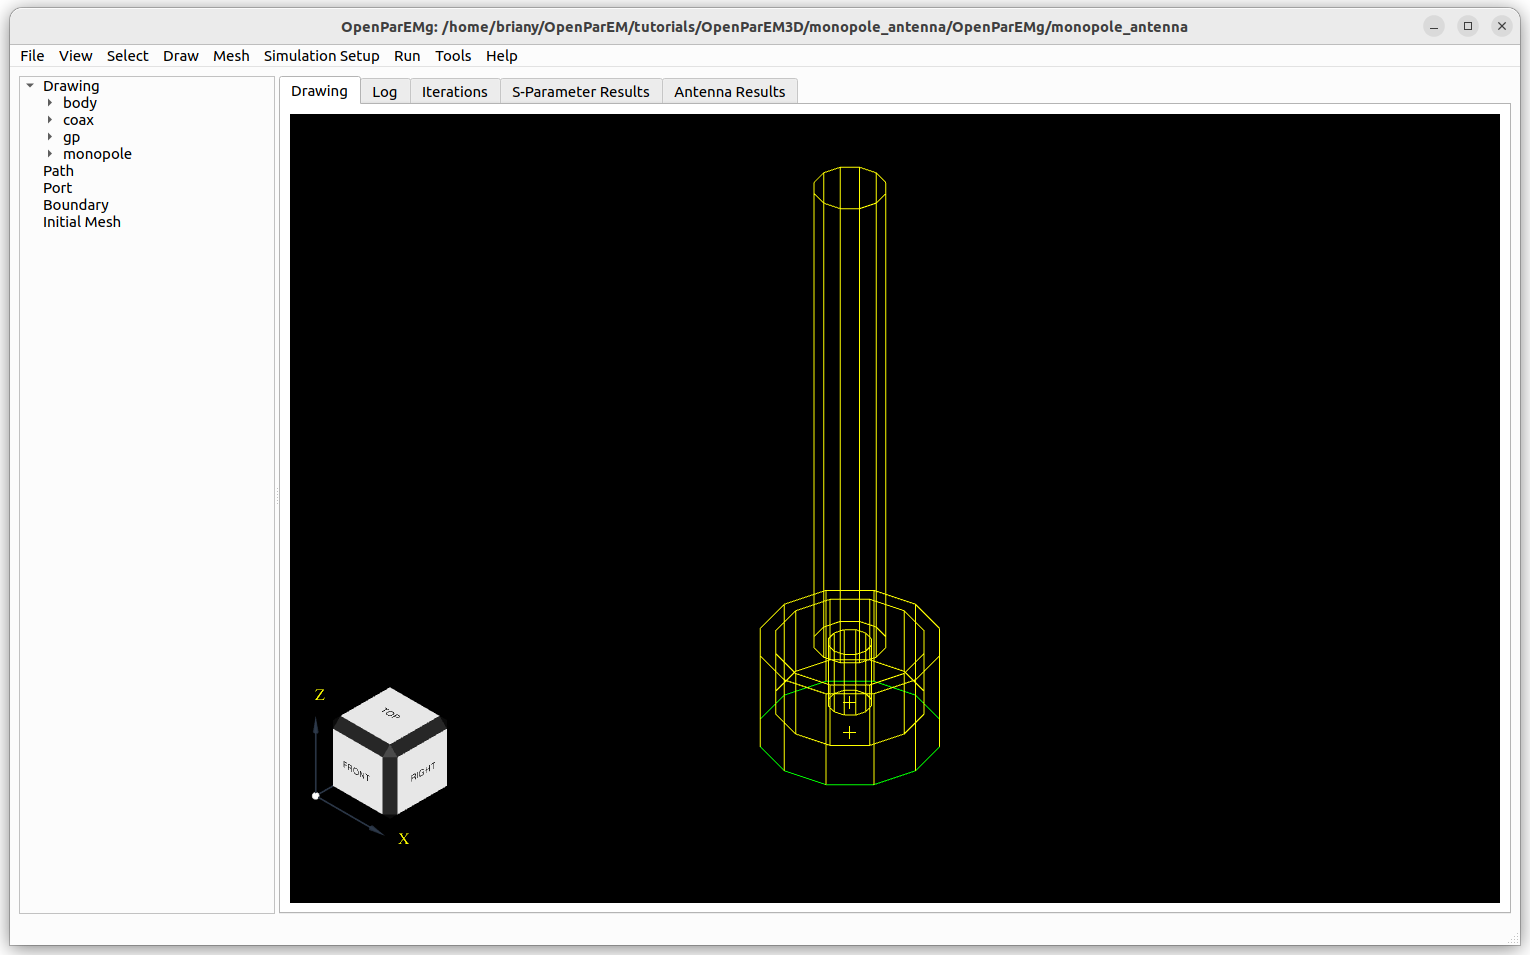
\includegraphics[width=0.75\textwidth]{../tutorials/OpenParEM3D/monopole_antenna/OpenParEMg/screenshots/monopole_zoom}
  \caption{Zoom of the coax feed and monopole antenna.}
  \label{fig:monopole_zoom}
\end{figure}
\item The final required structure is the air surrounding the antenna.
\item Draw a rectangle of any size, then edit it to set the position to X=-100, Y=-100, Z=100, and width=200 and height=200.  Extrude it 200~mm and rename it \texttt{air}.
\item Finish the creation of the metals by subtracting \texttt{body} from \texttt{air}, then \texttt{gp} from that result, then \texttt{monopole} from that result.  Rename the final object \texttt{air-metal}.  The resulting selection tree is shown in Fig.~\ref{fig:monopole_tree}.
\begin{figure}[H]
  \centering
  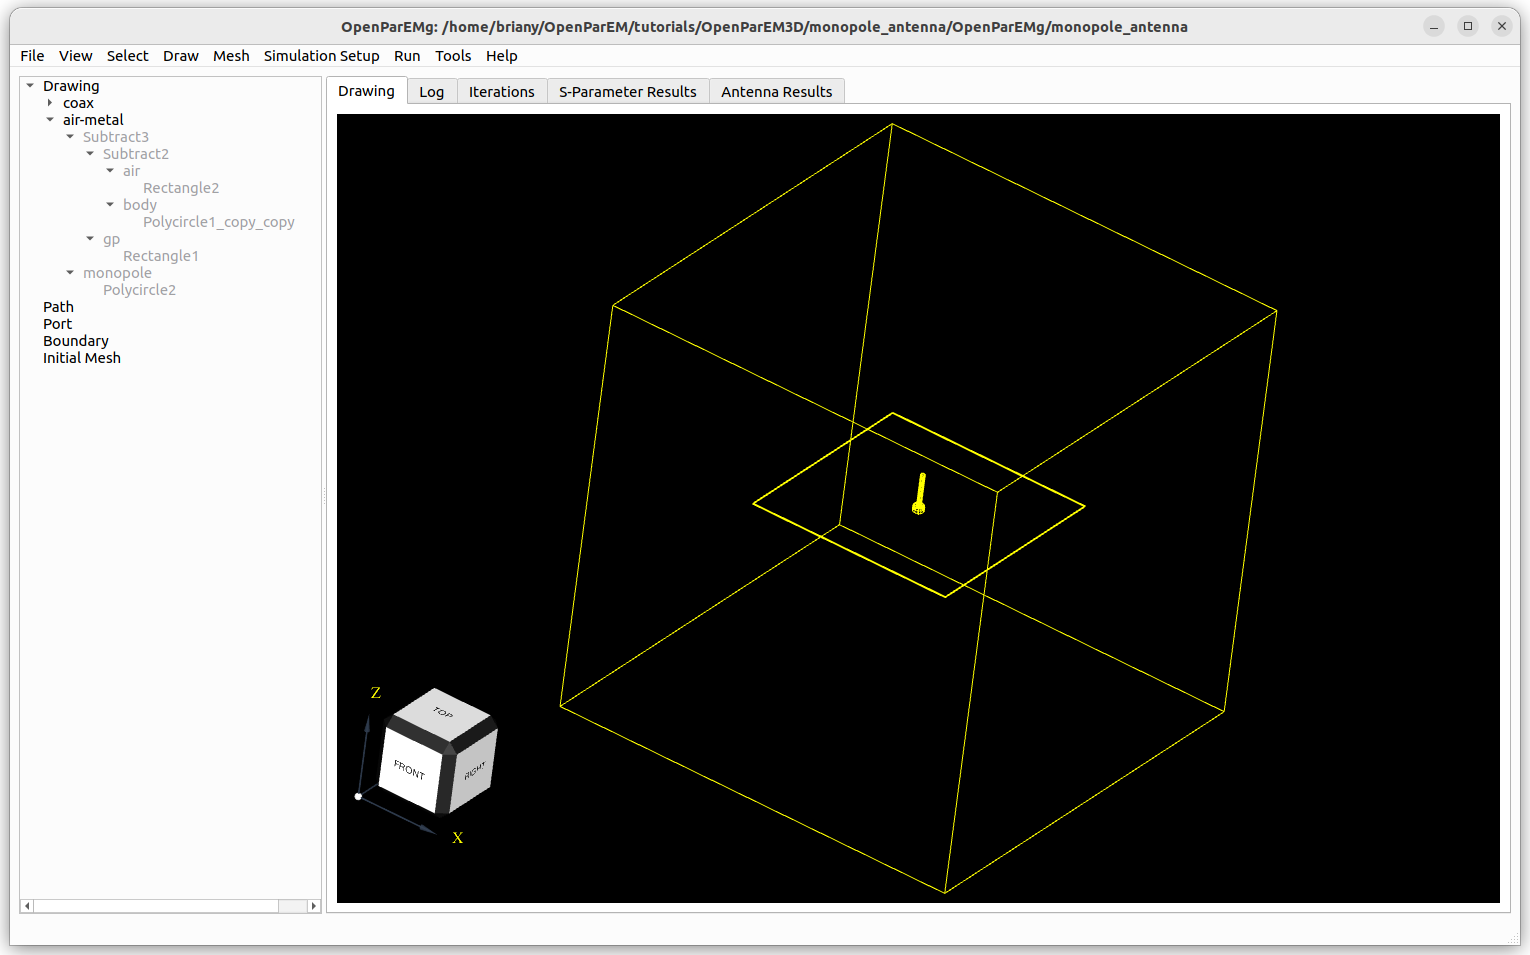
\includegraphics[width=0.75\textwidth]{../tutorials/OpenParEM3D/monopole_antenna/OpenParEMg/screenshots/monopole_tree}
  \caption{Selection tree after creating the metals through subtraction operations.}
  \label{fig:monopole_tree}
\end{figure}
\item OpenParEMg does not yet have mesh seeding to force additional meshing where it is known to be needed.  For a monopole, it is known that the fields at the tip of the monopole are very important, so manual seeding is desirable.  The corners of ground planes are also important.
\item Manual seeding can be implemented by adding lines and polylines to the drawing.  gmsh will imprint these onto the mesh, creating extra mesh elements where they are needed.  It is actually more conventient to add a rectangle or polycircle then convert these to polylines.
\item Expand the tree and select and copy the polycircle to forms the monopole extrusion.  Rename the new polycircle \texttt{dummy1}.  Edit the polycircle and chance the center position Z=17 and the radius to 3.
\item Copy this polycircle and edit the position to put it at Z=19.  Rename this polycircle \texttt{dummy2}.
\item Copy \texttt{dummy2} and change the radius to 1~mm.  Rename this polycircle \texttt{dummy3}.
\item Copy \texttt{dummy2} and \texttt{dummy3} and move the copies to $z$=13~mm.  Repeat to place two polycircles at $z$=9~mm and then two more at $z$=5~mm.
\item Copy \texttt{dummy2} then move the copy to the a corner of the ground plane.  Rename this polycircle \texttt{dummy4}.
\item Copy \texttt{dummy4} then move the copy to the other size of the same corner.  Rename this polycircle \texttt{dummy5}.
\item Select the two polycircles at this corner and copy them to the other three corners, renaming if desired.
\item Select the first dummy object then SHIFT-select the last dummy object.  Right click and click \texttt{Convert to Polyline}.
\item The final drawing with dummy objects added is shown in Fig.~\ref{fig:monopole_dummy}
\begin{figure}[H]
  \centering
  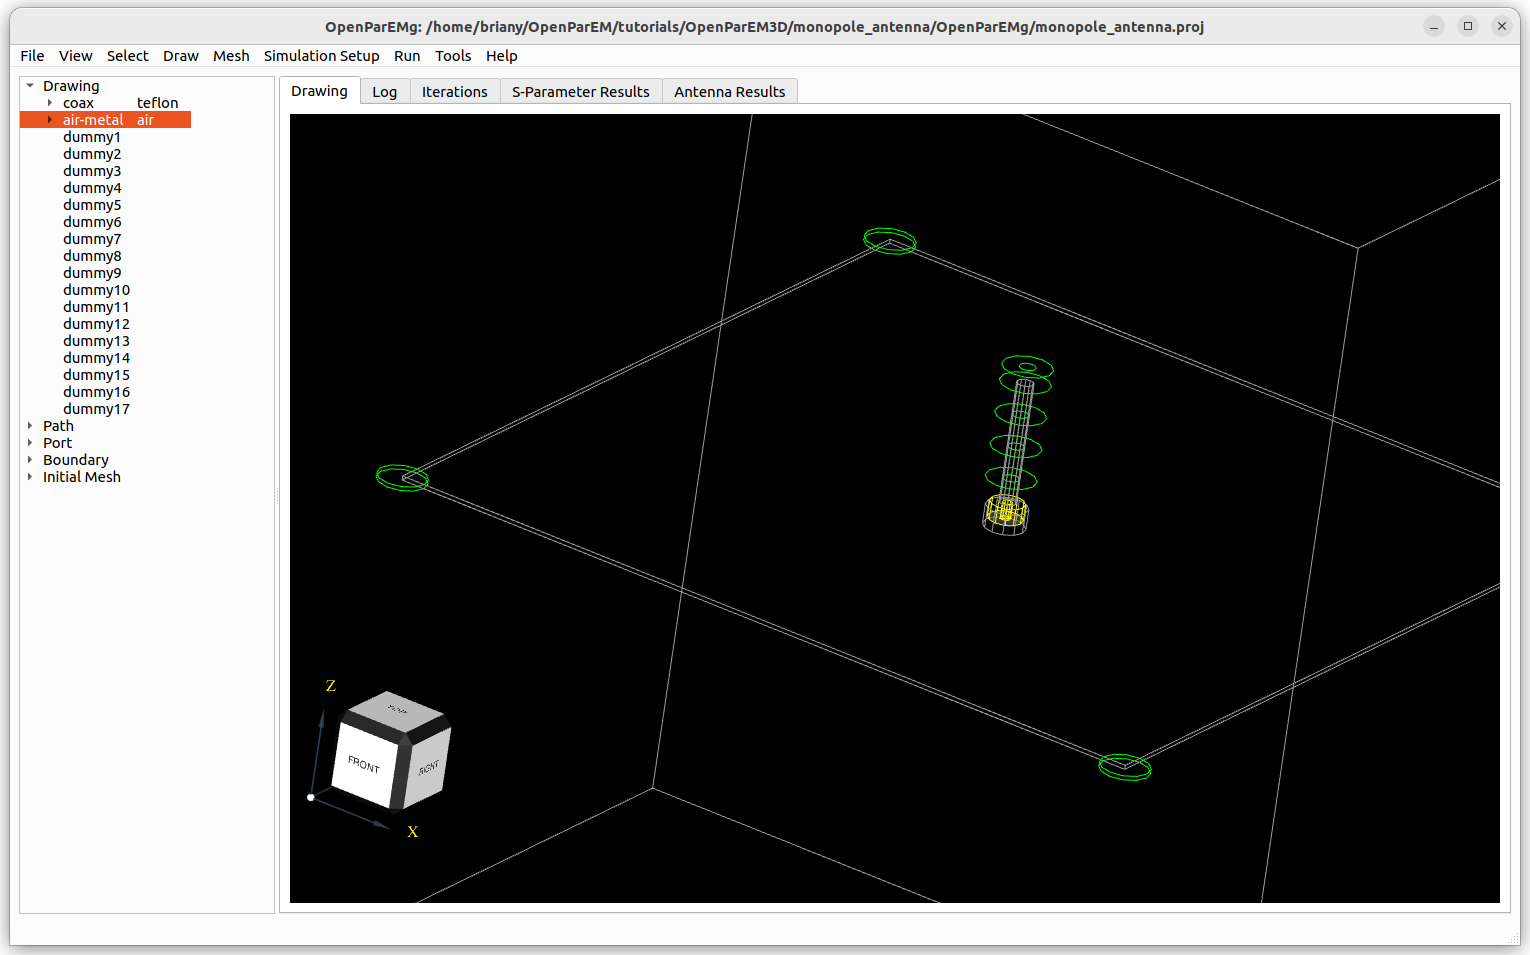
\includegraphics[width=0.75\textwidth]{../tutorials/OpenParEM3D/monopole_antenna/OpenParEMg/screenshots/monopole_dummy}
  \caption{Final structure with dummy polylines added for mesh seeding.}
  \label{fig:monopole_dummy}
\end{figure}

\end{itemize}

\subsubsection{Radiation Boundaries}

\begin{itemize}
\item Select \texttt{Select}$\rightarrow$\texttt{Face}, then click an outer face of \texttt{air-metal}, then CTRL-click the other two outer visible faces.
\item Right click, then click \texttt{Create Boundary}. The default boundary is a radiation boundary.
\item Rotate the drawing, then create boundaries for the other three outer faces.
\item When complete, a size-sided blue cube should be visible that hides all interior detail as shown in Fig.~\ref{fig:monopole_radiation}.
\begin{figure}[H]
  \centering
  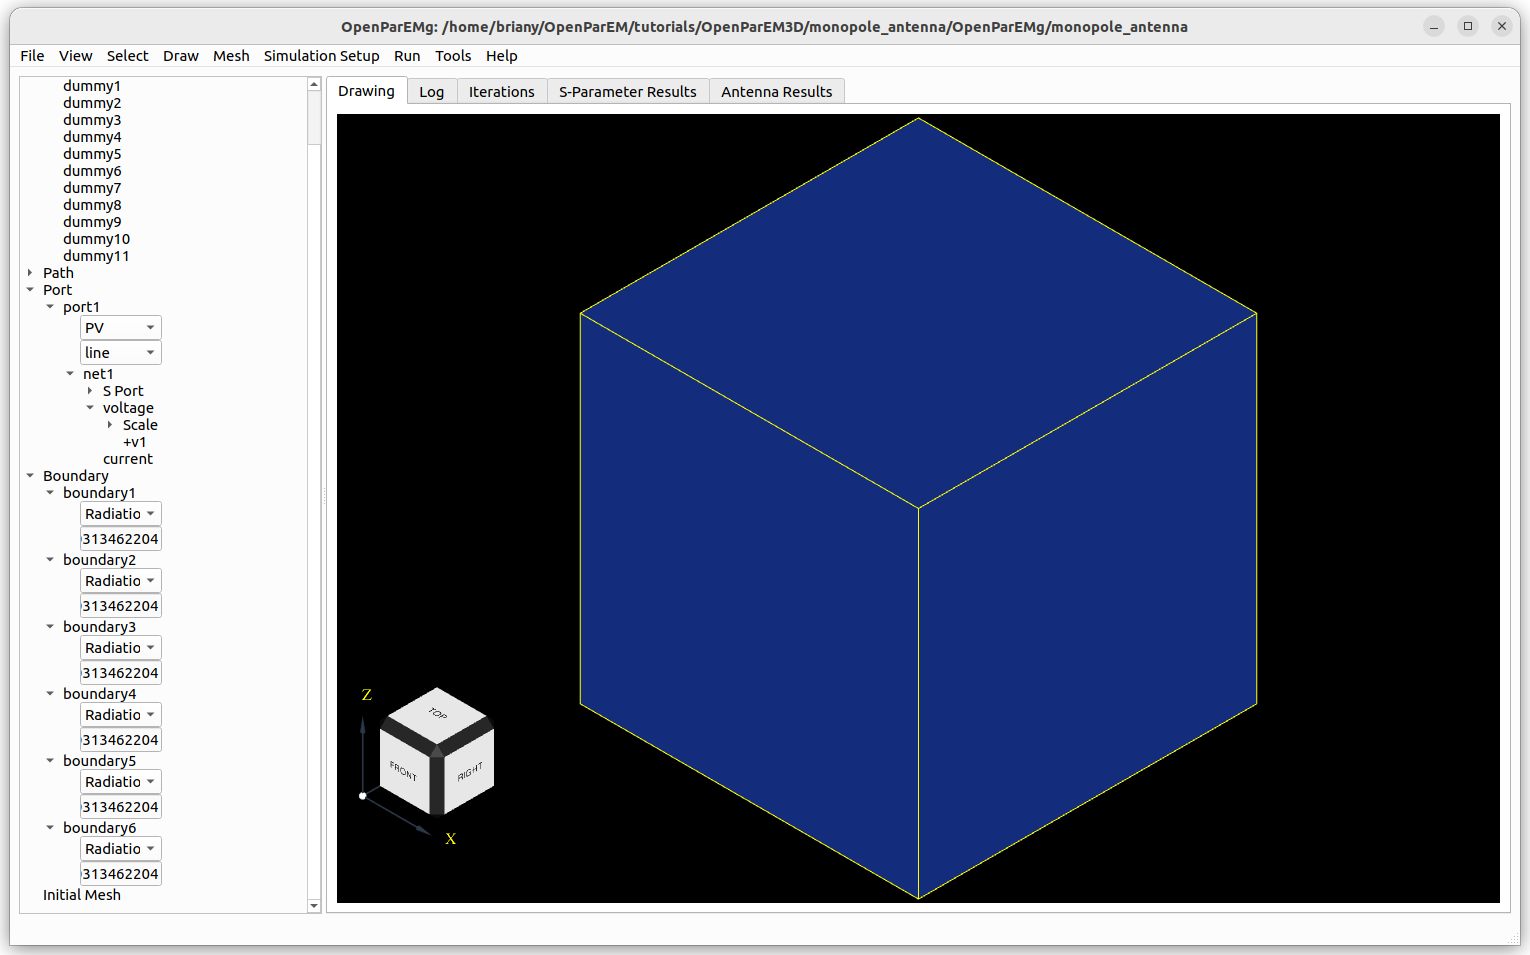
\includegraphics[width=0.75\textwidth]{../tutorials/OpenParEM3D/monopole_antenna/OpenParEMg/screenshots/monopole_radiation}
  \caption{View with adiation boundaries applied.}
  \label{fig:monopole_radiation}
\end{figure}
\end{itemize}

\subsubsection{Ports}

\begin{itemize}

\item Rotate the drawing to view the coax with the monopole on the far side.
\item Select \texttt{air-metal}, right click, and click \texttt{Hide}.
\item Zoom in to the \texttt{item}.
\item Select \texttt{Select}$\rightarrow$\texttt{Face}, then click on the face of the coax.
\item Right click and click \texttt{Create Port}.
\item Add a voltage integration line from the outer conductor to the inner conductor.
\item The final port is shown in Fig.~\ref{fig:monopole_port}
\begin{figure}[H]
  \centering
  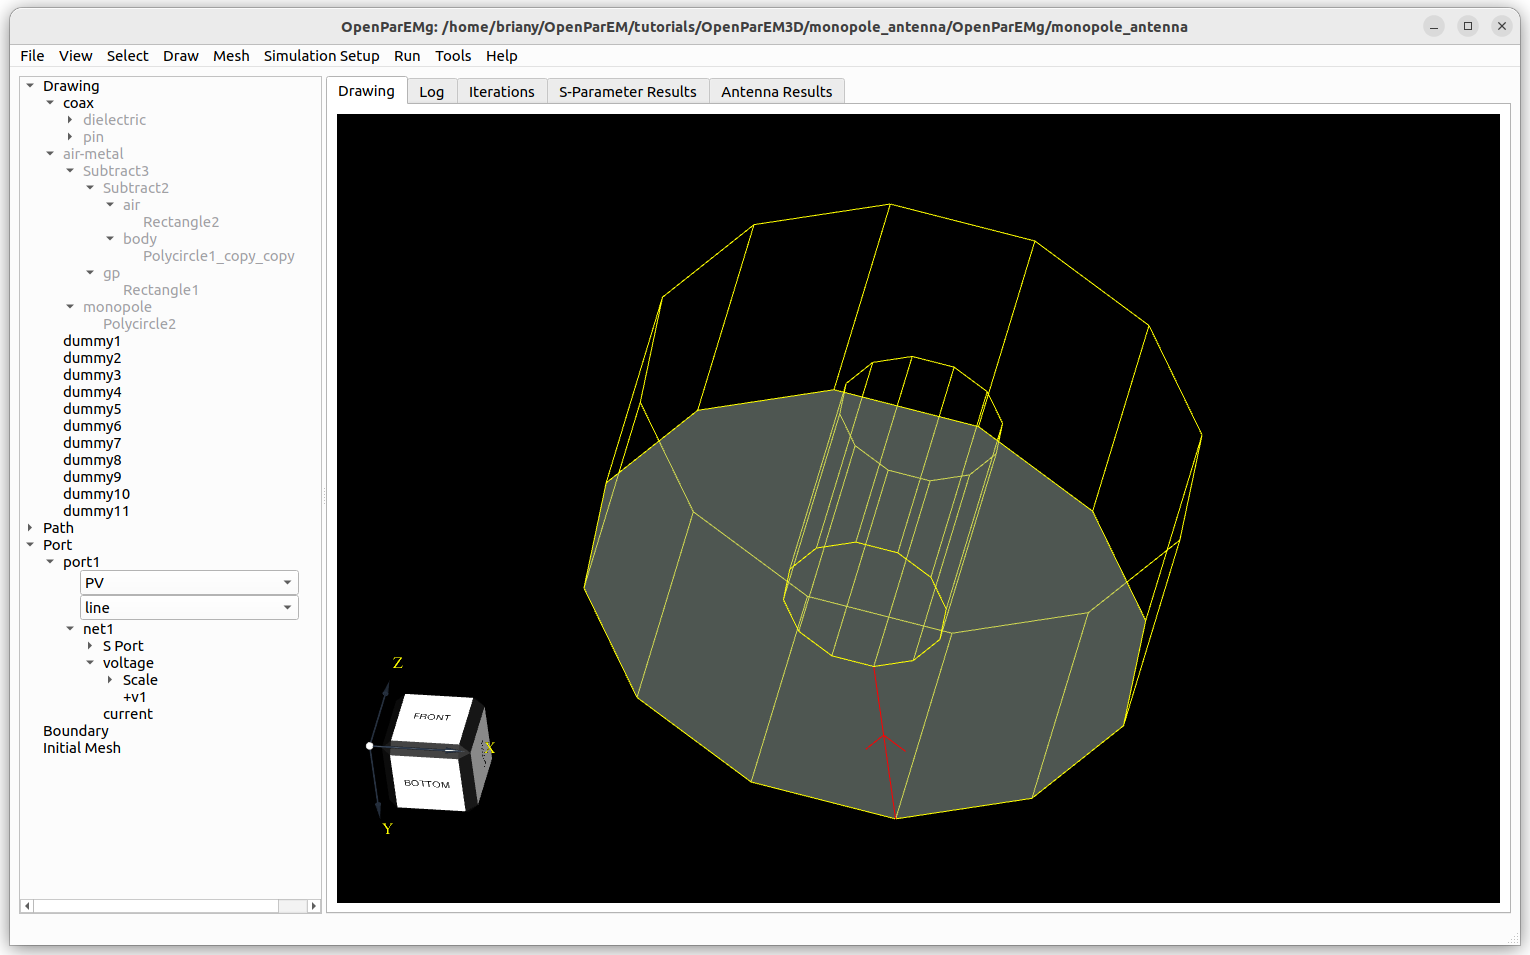
\includegraphics[width=0.75\textwidth]{../tutorials/OpenParEM3D/monopole_antenna/OpenParEMg/screenshots/monopole_port}
  \caption{Coaxial port with voltage integration line.}
  \label{fig:monopole_port}
\end{figure}
\end{itemize}

\subsubsection{Materials}

\begin{itemize}

\item Create the materials file \texttt{local\_materials.txt} in any text editor and set the text contents to
\begin{Verbatim}[fontsize=\small]
#OpenParEMmaterials 1.0
Material
   name=air
   type=dielectric
   Temperature
      temperature=any
      Frequency
         frequency=any
         er=1.0006
         mur=1
         tand=0
         Rz=0
      EndFrequency
   EndTemperature
   Source
      Constantine A. Balanis, "Advanced Engineering Electromagnetics",
      John Wiley and Sons, 1989, p.79.
   EndSource
EndMaterial

Material
   name=teflon
   Temperature
      temperature=any
      Frequency
         frequency=any
         er=2.2
         mur=1
         tand=0.0
         Rz=0
      EndFrequency
   EndTemperature
   Source
      generic teflon
   EndSource
EndMaterial
\end{Verbatim}

\item Set the local materials to this file in the materials editor at \texttt{Simulation Setup}$\rightarrow$\texttt{Materials ...}.
\item Select \texttt{coax}, right click, click \texttt{Assign Material}, and select \texttt{teflon}.
\item Assign \texttt{air} to \texttt{air-metal}.
\end{itemize}

\subsubsection{Mesh}

\begin{itemize}
\item Generate the mesh, which should look like the mesh in Fig.~\ref{fig:monopole_mesh}.
\begin{figure}[H]
  \centering
  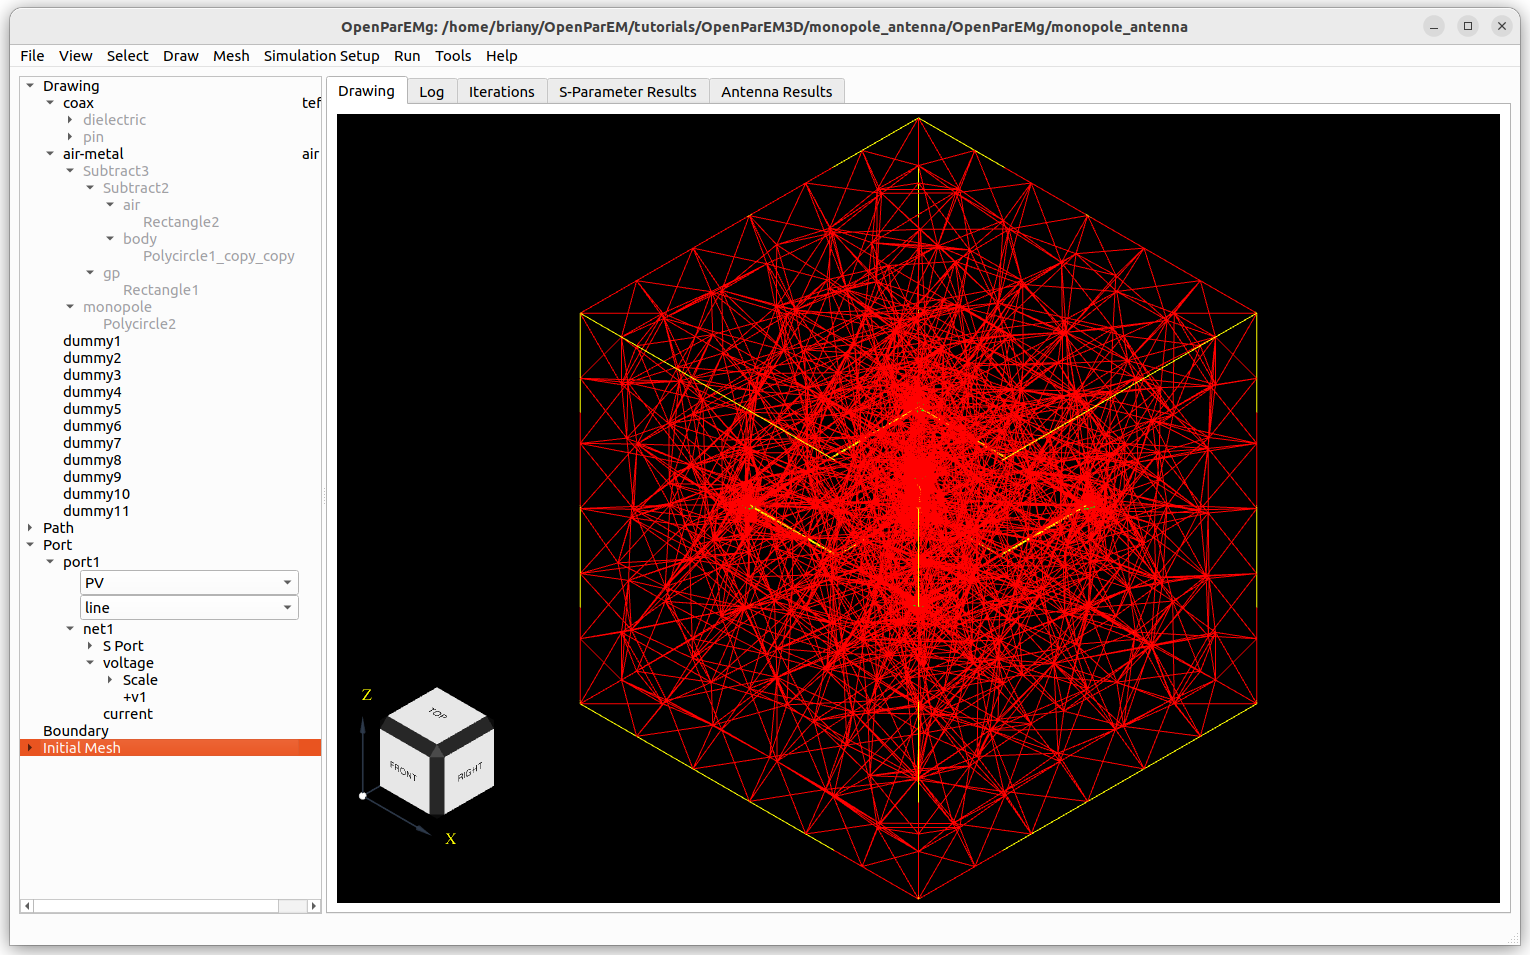
\includegraphics[width=0.75\textwidth]{../tutorials/OpenParEM3D/monopole_antenna/OpenParEMg/screenshots/monopole_mesh}
  \caption{Mesh for the mononpole dipole}
  \label{fig:monopole_mesh}
\end{figure}
\item In \texttt{Mesh}$\rightarrow$\texttt{Options ...}, set the \texttt{Quality Limit} to 1000000.
\end{itemize}


\subsubsection{Simulation Setup}

\begin{itemize}
\item Select \texttt{Simulation Setup}$\rightarrow$\texttt{Options ...}.
\item On the \texttt{S-Parameters} tab, uncheck \texttt{Normalize}.
\item On the \texttt{Controls} tab, set the \texttt{FEM Order} to 3, and pick a value for \texttt{Parallel Processing Slot Count}.  If using MPICH, unceck \texttt{Oversubscribe}.
\item On the \texttt{Outputs} tab, check \texttt{Save 3D Fields}.
\item Select \texttt{Simulation Setup}$\rightarrow$\texttt{Frequency Plan ...}, then add two frequencies to solve at 4.7 and 5~GHz.  Adaptive mesh refinement will occur at 5~GHz.  A prior frequency sweep (not shown) shows the minimum return loss at 4.7~GHz.  Setting adaptive meshing to occur at 5~GHz helps prevent excessive mesh refinement compared to refinement at the resonant frequency, where small changes to the mesh can cause large changes to the S-parameters that prevent convergence on tight convergence criteria.
\item Select \texttt{Simulation Setup}$\rightarrow$\texttt{Refinement ...}, change \texttt{Relative S} to 0.01 and \texttt{Absolute H} to 1e-06.
\item Select \texttt{Simulation Setup}$\rightarrow$\texttt{Antenna Patterns ...}, click \texttt{Add}, then change \texttt{Latitude} to 15.
\item Add a second 2D pattern by clicking \texttt{Add}, then change \texttt{Plane} to \texttt{xz} and \texttt{Rotation} to 180.
\item Click \texttt{Ok}.
\item Save the project.
\end{itemize}

\subsubsection{Solving}

\begin{itemize}
\item Select \texttt{Run}$\rightarrow$\texttt{Run}.  If the \texttt{Run} option is grayed out, then a step was somehow missed along the way.  Hover over the \texttt{Run}$\rightarrow$\texttt{Run} menu item to get a list of what needs to be done to enable the run to be started.
\item Review the tabs to monitor the job. This project runs much slower than the other tutorials.
\item The calculated S-parameters are shown in Fig.~\ref{fig:monopole_sparameters}, while the calculated antenna parameters are shown in Fig.~\ref{fig:monopole_gain}.  Due to iterative solution of the matrices when using MPI and iterative mesh refinement, the results change slightly from run to run.
\begin{figure}[H]
  \centering
  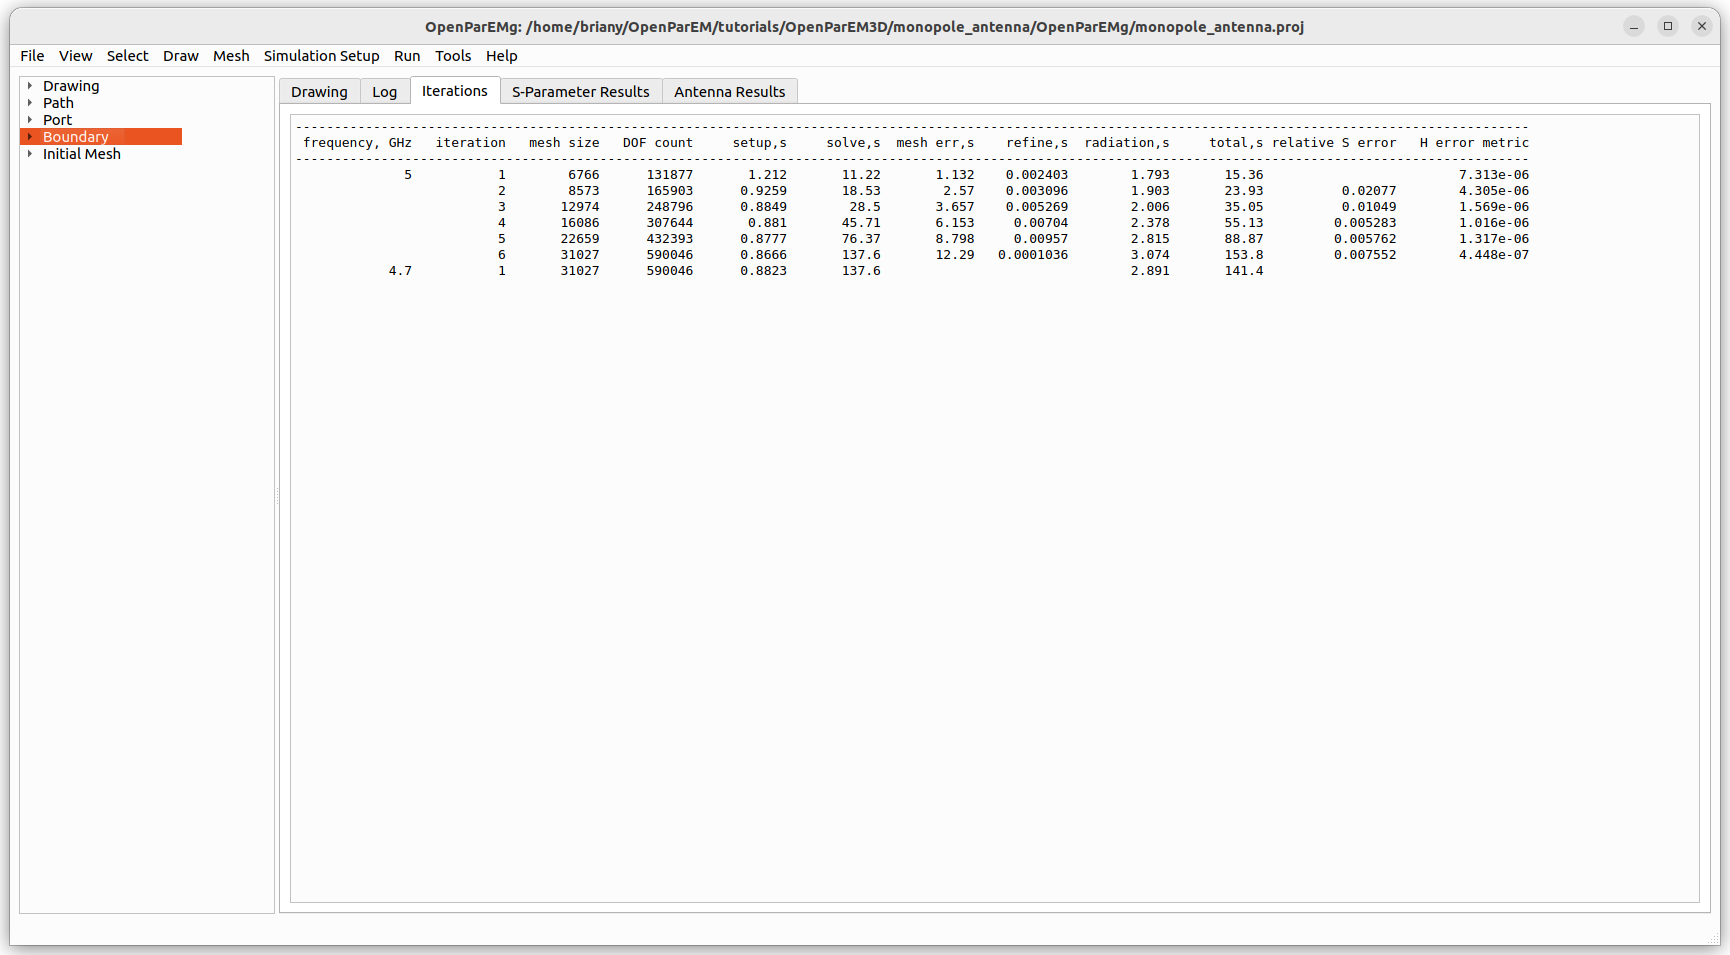
\includegraphics[width=0.75\textwidth]{../tutorials/OpenParEM3D/monopole_antenna/OpenParEMg/screenshots/monopole_sparameters}
  \caption{S-parameters for the monopole antenna.}
  \label{fig:monopole_sparameters}
\end{figure}
\begin{figure}[H]
  \centering
  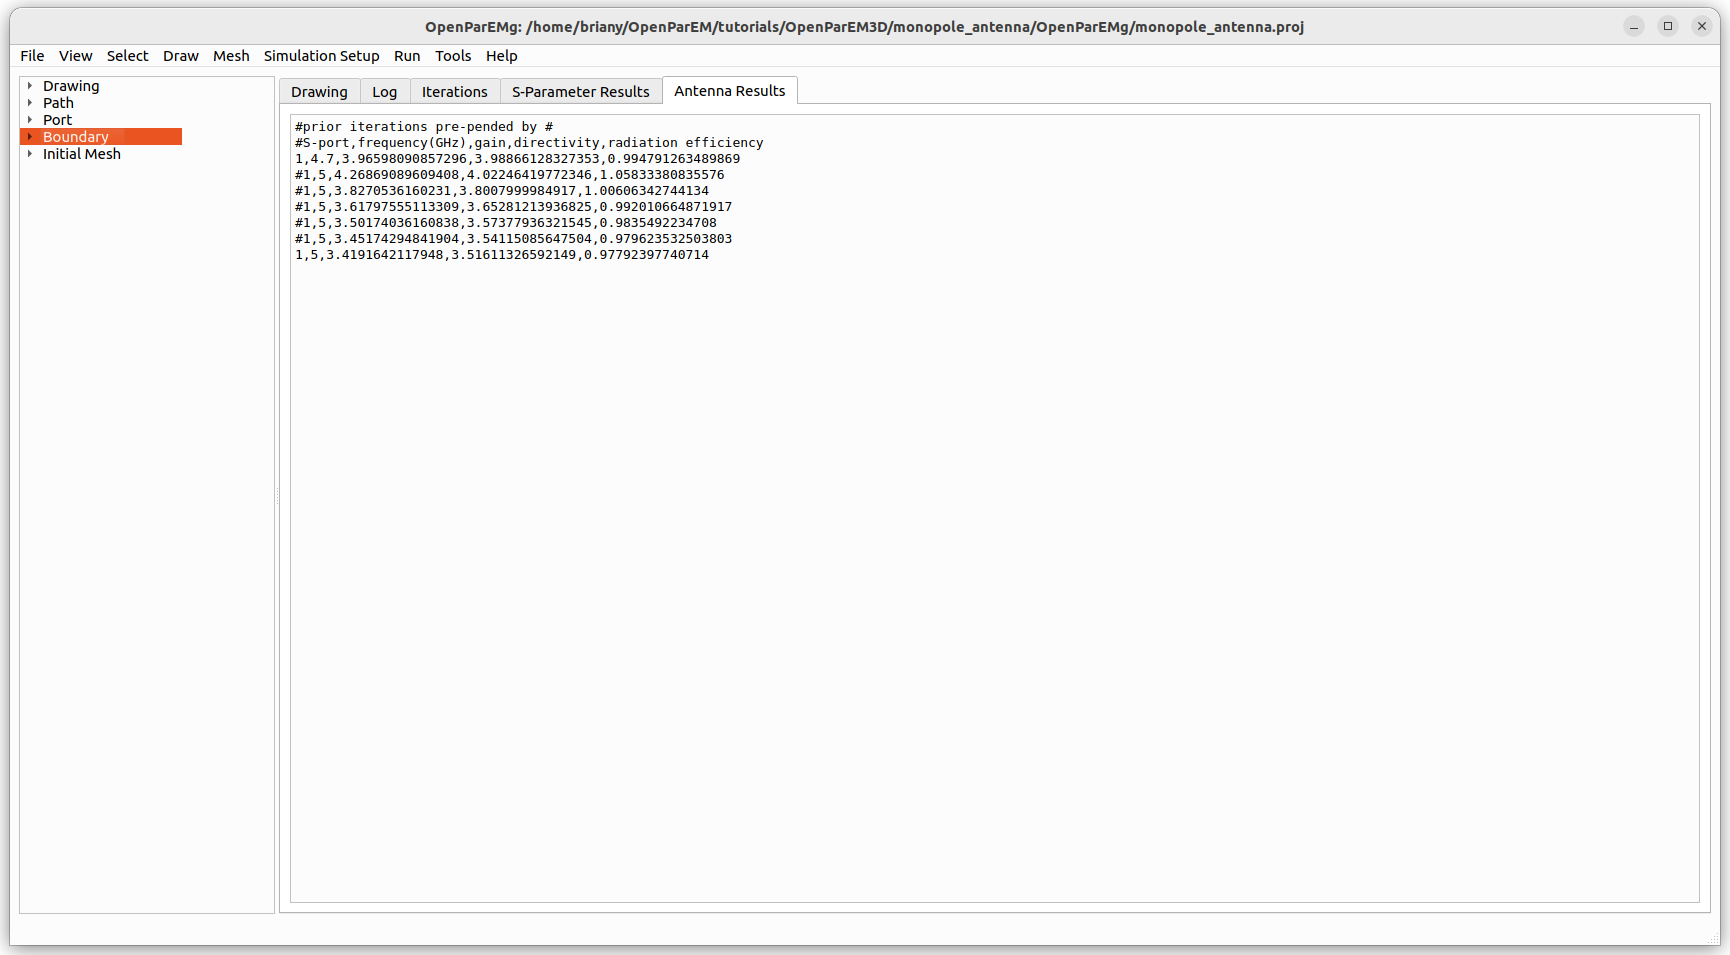
\includegraphics[width=0.75\textwidth]{../tutorials/OpenParEM3D/monopole_antenna/OpenParEMg/screenshots/monopole_gain}
  \caption{Antenna metrics for the mononpole dipole}
  \label{fig:monopole_gain}
\end{figure}
\end{itemize}

\subsubsection{3D Plots}

\begin{itemize}

\item View the computed far fields with ParaView using the files saved in the directory \texttt{ParaView\_monopole\_antenna\_FarField}.
Open the file \texttt{G\_4.7e+09\_SP1}, change \texttt{Solid Color} to \texttt{G}, set \texttt{Normal Array} to \texttt{normals}, and set \texttt{Specular} to \texttt{1}.  The 3D far-field gain is shown in Fig.~\ref{fig:monopole_G}(a), where the influence of the finite ground plane can be seen on the field.

\begin{figure}[H]
  \centering
  \begin{subfigure}{0.33\textwidth}
     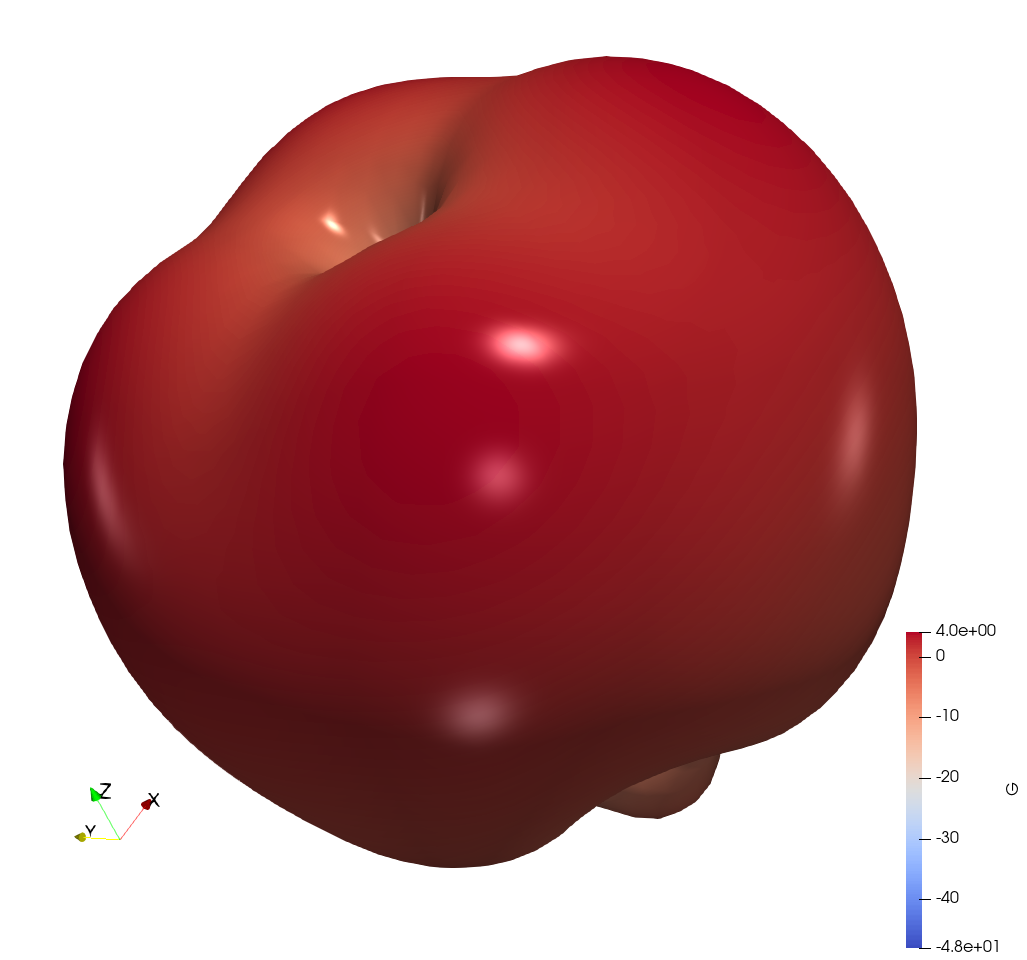
\includegraphics[width=\linewidth]{../tutorials/OpenParEM3D/monopole_antenna/OpenParEMg/screenshots/monopole_G}
     \caption{Isotropic gain.}
  \end{subfigure}
  \begin{subfigure}{0.33\textwidth}
     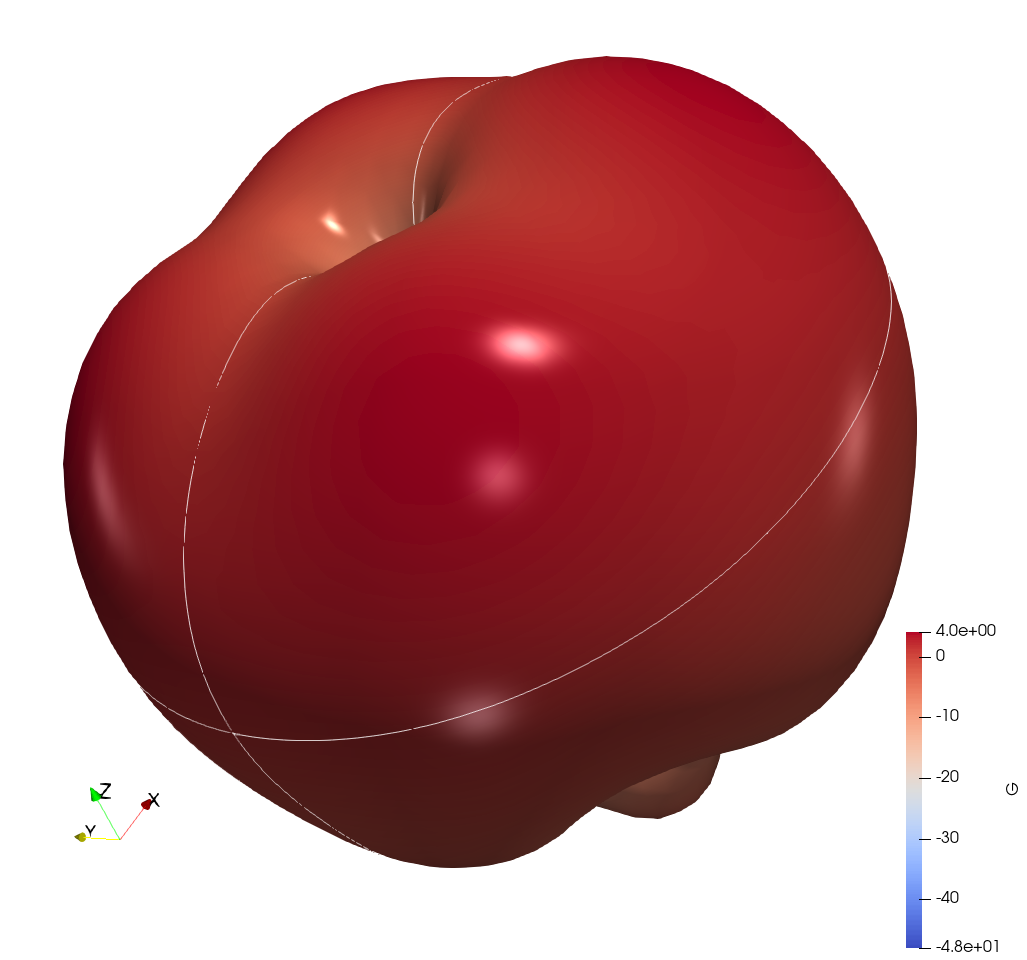
\includegraphics[width=\linewidth]{../tutorials/OpenParEM3D/monopole_antenna/OpenParEMg/screenshots/monopole_G_slices}
     \caption{Isotropic gain with slices.}
  \end{subfigure}
  \caption{Isotropic gain at 4.7 GHz.}
  \label{fig:monopole_G}
\end{figure}

\item Open the files \texttt{slice\_G\_4.7e+09\_xz\_0\_0\_SP1} and \texttt{slice\_G\_4.7e+09\_xz\_0\_0\_SP1} to show slices cut through the 3D pattern as shown in Fig.~\ref{fig:monopole_G}(b).  View all together to ensure that the slices are as expected, and de-select various plots to explore the slices in isolation.

\end{itemize}

\subsubsection{2D Plots}

\begin{itemize}

\item Reports for the slices are in the directory \texttt{Report\_monopole\_antenna\_FarField}.  These can be viewed by executing
\begin{Verbatim}[fontsize=\small]
   $ evince radiation_pattern_G_4.7e+09_xy_15_0_SP1.pdf &
   $ evince radiation_pattern_G_4.7e+09_xz_0_0_SP1.pdf &
\end{Verbatim}
\noindent The reports are shown in Fig.~\ref{fig:monopole_G_slices}.  Note that the gains and directivities shown on the slice report are the maximum values on that slice.  The maximum values for the 3D pattern overall are given in the far-field results file, \texttt{monopole\_antenna\_fields\_FarField\_results.csv} for this project.

\begin{figure}[H]
  \centering
  \begin{subfigure}{0.408\textwidth}
     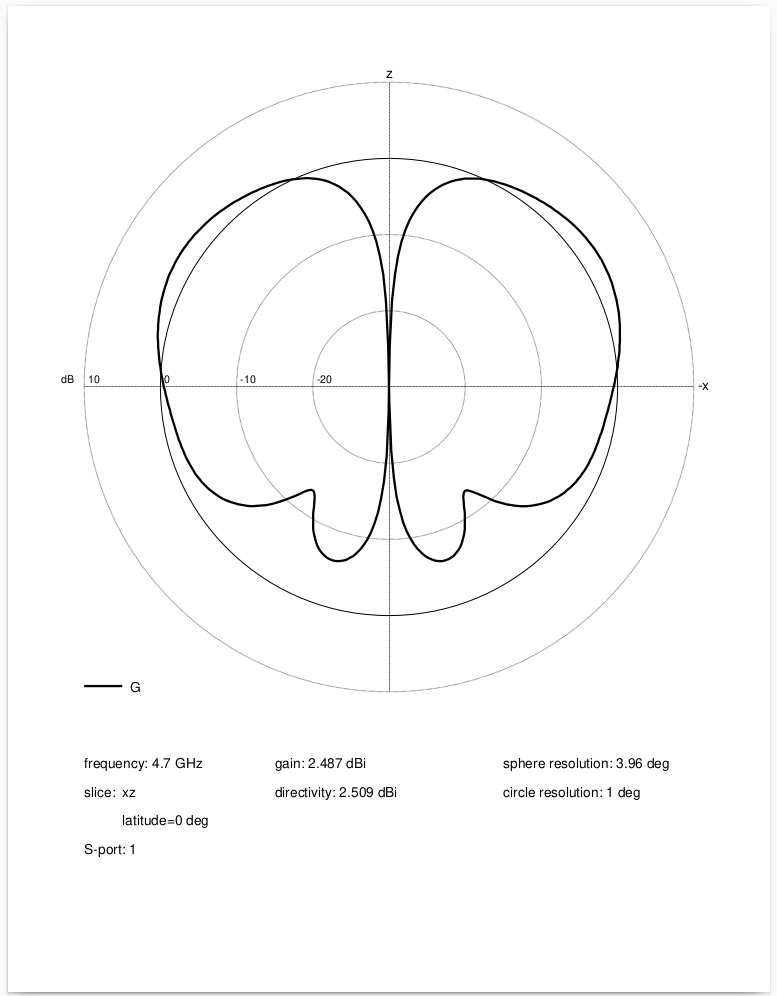
\includegraphics[width=\linewidth]{../tutorials/OpenParEM3D/monopole_antenna/OpenParEMg/screenshots/radiation_pattern_G_4.7e+09_xz_0_180_SP1}
     \caption{Slice through the x-z plane.}
  \end{subfigure}
  \begin{subfigure}{0.41\textwidth}
     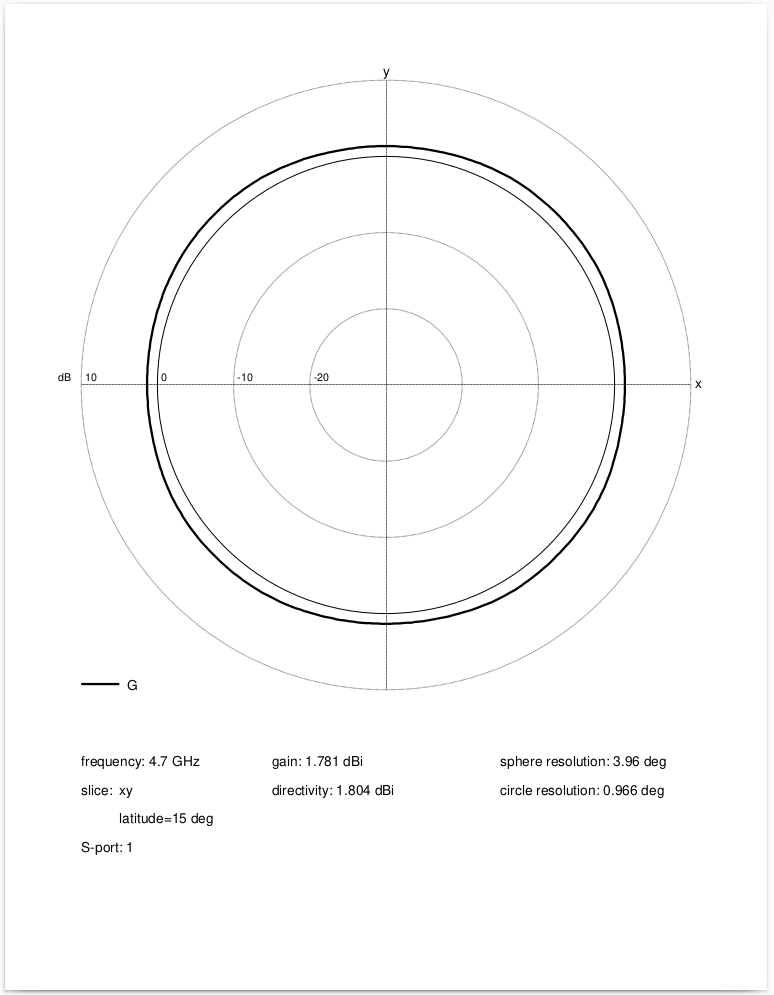
\includegraphics[width=\linewidth]{../tutorials/OpenParEM3D/monopole_antenna/OpenParEMg/screenshots/radiation_pattern_G_4.7e+09_xy_15_0_SP1}
     \caption{Slice through the x-y plane at latitude 15$^\circ$.}
  \end{subfigure}
  \caption{Isotropic gain slice reports at 4.7 GHz.}
  \label{fig:monopole_G_slices}
\end{figure}

\item 2D field plots throughout the 3D volume can be set up and viewed in ParaView.  Taking slices through the volume, the real part of the electric field computed at 4.7~GHz on the x-z plane is shown in Fig.~\ref{fig:monopole_ReE}, while Fig.~\ref{fig:monopole_ReH} shows the real part of the magnetic field on the x-y plane at 4~mm above the ground plane.

\begin{figure}[H]
  \centering
  \begin{subfigure}{0.6\textwidth}
     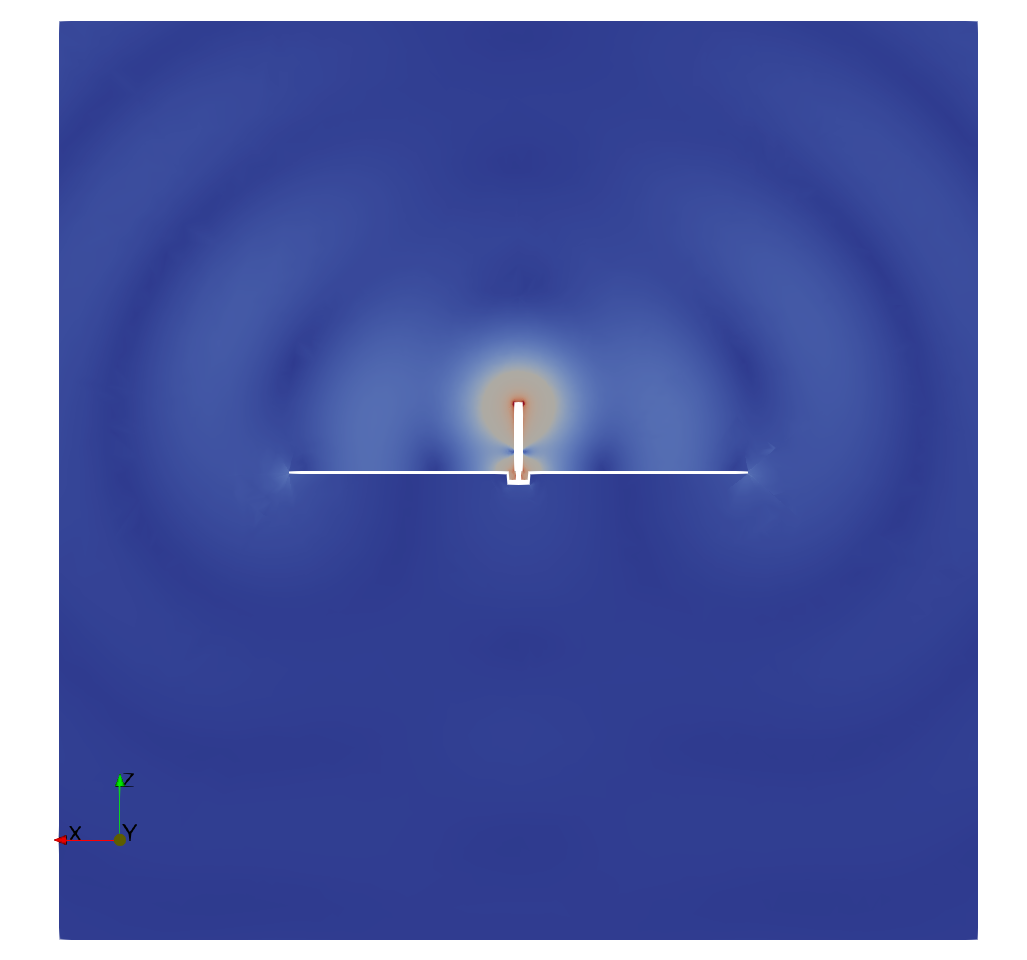
\includegraphics[width=\linewidth]{../tutorials/OpenParEM3D/monopole_antenna/OpenParEMg/screenshots/monopole_ReE}
     \caption{$|\textnormal{Re}(\overline{E})|$}
  \end{subfigure}
  \par\bigskip
  \begin{subfigure}{0.6\textwidth}
     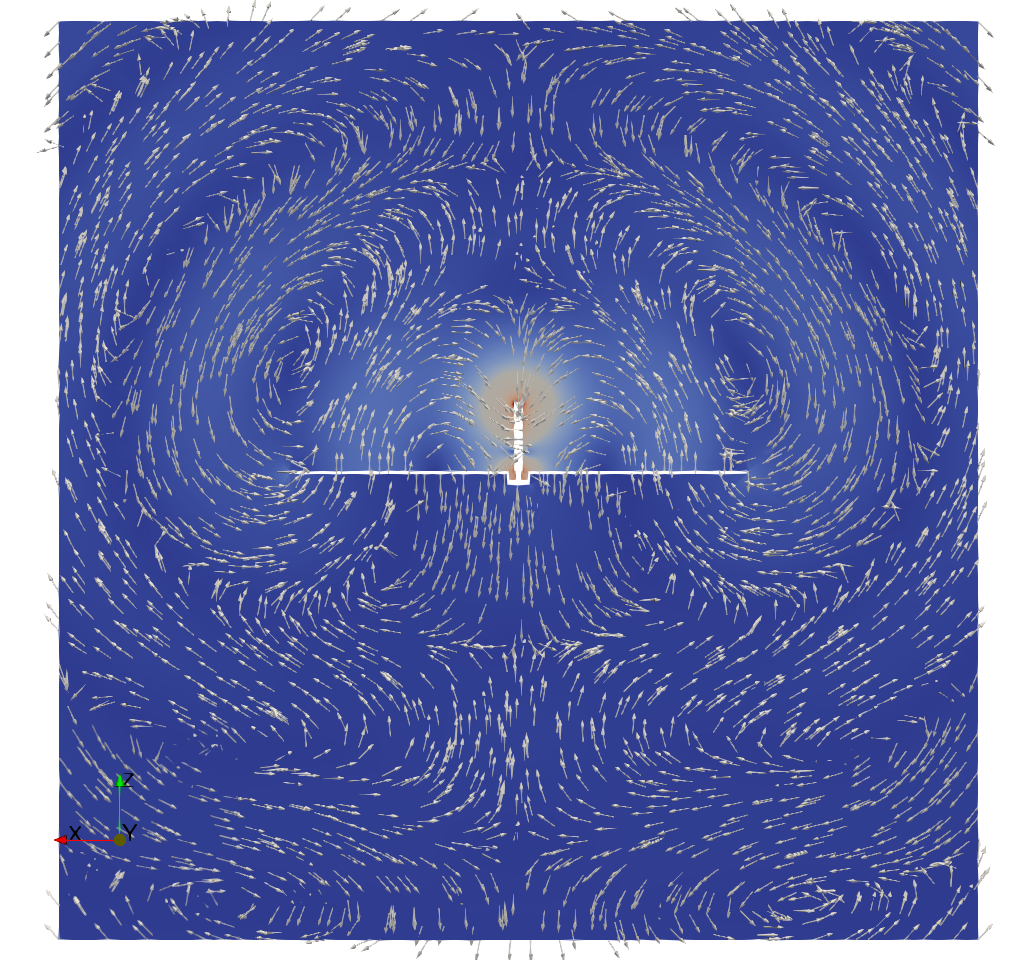
\includegraphics[width=\linewidth]{../tutorials/OpenParEM3D/monopole_antenna/OpenParEMg/screenshots/monopole_vector_ReE}
     \caption{$\textnormal{Re}(\overline{E})$}
  \end{subfigure}
  \caption{Real part of the electric field at 4.7~GHz.}
  \label{fig:monopole_ReE}
\end{figure}
\begin{figure}[H]
  \centering
  \begin{subfigure}{0.6\textwidth}
     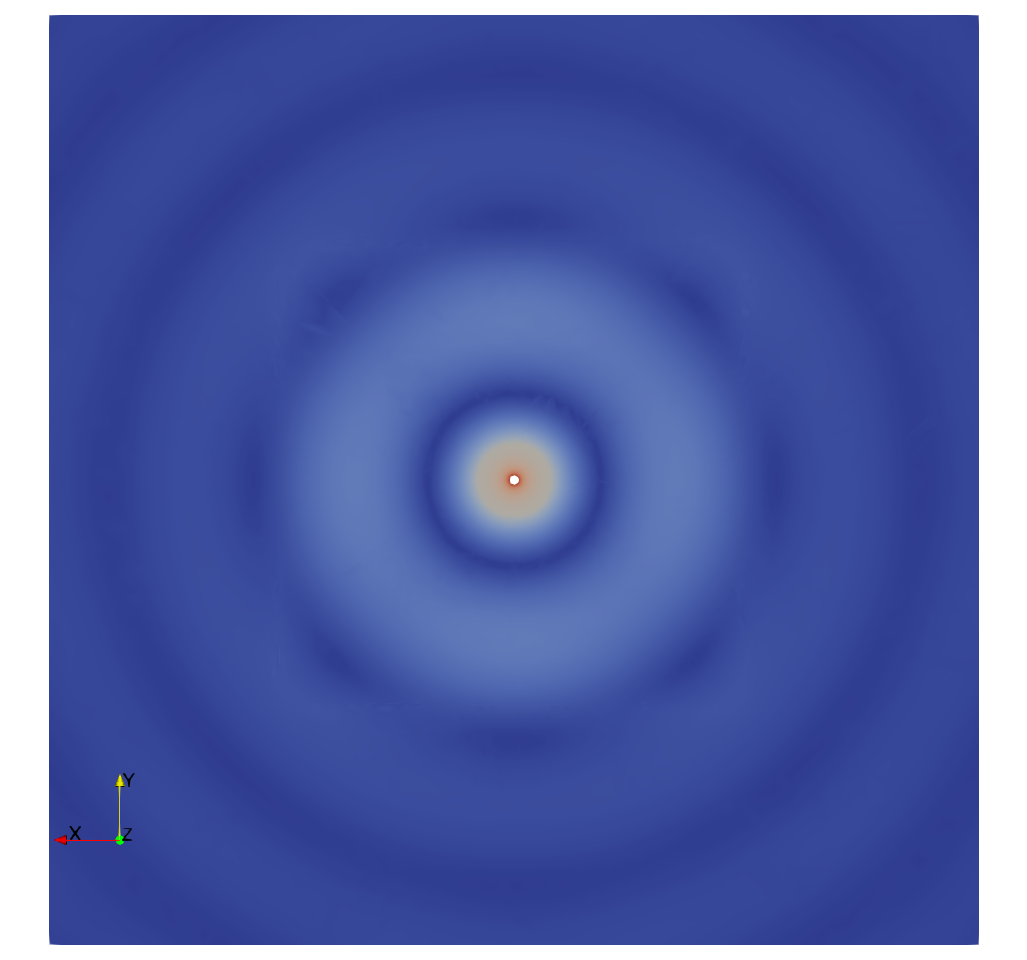
\includegraphics[width=\linewidth]{../tutorials/OpenParEM3D/monopole_antenna/OpenParEMg/screenshots/monopole_ReH}
     \caption{$|\textnormal{Re}(\overline{H})|$}
  \end{subfigure}
  \par\bigskip
  \begin{subfigure}{0.6\textwidth}
     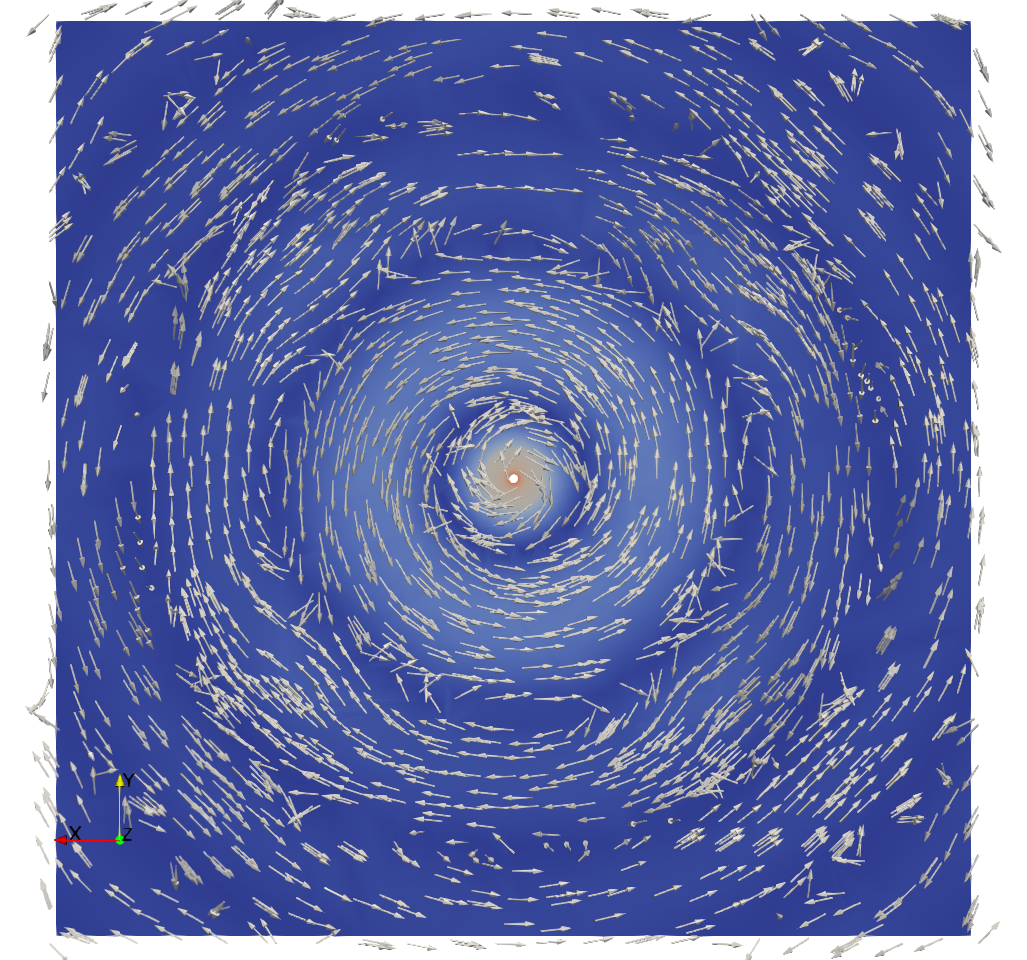
\includegraphics[width=\linewidth]{../tutorials/OpenParEM3D/monopole_antenna/OpenParEMg/screenshots/monopole_vector_ReH}
     \caption{$\textnormal{Re}(\overline{H})$}
  \end{subfigure}
  \caption{Real part of the magnetic field at 4.7~GHz.}
  \label{fig:monopole_ReH}
\end{figure}

\end{itemize}


\section{Techniques}

The section \texttt{Techniques} in the users manual "OpenParEM3D\_Users\_Manual.pdf" should be reviewed.

\appendix

\newpage
\section{Drawing File Format Specification}
\label{sec:drawing_file_spec}


\begin{Verbatim}[fontsize=\small]
#OpenParEMgDrawing 1.0 // required on first real line

// a comment

// Each item represents one physical structure in the drawing and is shown in the item tree.

// 2D primitives

Line
   name=text
   point=(double,double,double)     // (x,y,z) coordinate in m
   point=(double,double,double)     // (x,y,z) coordinate in m
   normal=(double,double,double)    // normal to the line (i.e. normal to the drawing plane)
   reverse={true|false}             // reverse the direction for extrusion
EndLine

// polylines must lie on a plane
// a closed polyline has point[0]=point[N-1]
Polyline
   name=text
   point=(double,double,double)     // (x,y,z) coordinate in m
      ...
   point=(double,double,double)     // (x,y,z) coordinate in m
   normal=(double,double,double)    // normal to the polyline (i.e. normal to the drawing plane)
   reverse={true|false}             // reverse the direction for extrusion of closed polylines
EndPolyline

Polycircle
   name=text
   N=integer                        // number of vertices
   center=(double,double,double)    // (x,y,z) coordinate of the center in m
   point=(double,double,double)     // (x,y,z) coordinate of the first point on the circle in m
   normal=(double,double,double)    // normal to the polycircle (i.e. normal to the drawing plane)
   reverse={true|false}             // reverse the direction for extrusion
EndPolycircle

Rectangle
   name=text
   origin=(double,double,double)    // (x,y,z) coordinate in m
   width=double                     // width in m
   height=double                    // height in m
   u=(double,double,double)         // (x,y,z) vector direction for u
   v=(double,double,double)         // (x,y,z) vector direction for v
   normal=(double,double,double)    // normal to the rectangle (i.e. normal to the drawing plane)
   reverse={true|false}             // reverse the direction for extrusion
EndRectangle

// 3D operations 

// extrude requires one 2D primitive child 
Extrude
   name=text
   [material=text]  // valid if not nested
   length=double;   // extrusion length in m

   Item             // 2D primitive polyline (closed), polycircle, or rectangle
      ...
   EndItem
EndExtrude

// merge requires two children
Merge
   name=text
   [material=text]  // valid if not nested

   Item             // extrude, merge, subtract, or SOLID or COMPOUND Brep; implies nesting
      ...
   EndItem

   Item             // extrude, merge, subtract, or SOLID or COMPOUND Brep; implies nesting
      ...
   EndItem
EndMerge

// subtract requires two children 
Subtract
   name=text
   [material=text]  // valid if not nested

   Item             // extrude, merge, subtract, or SOLID or COMPOUND Brep; implies nesting
      ...
   EndItem

   Item             // extrude, merge, subtract, or SOLID or COMPOUND Brep; implies nesting
      ...
   EndItem
EndSubtract

BRep
   name=text
   [material=text]  // valid if not nested

   text             // definining the Brep
EndBRep

// any number of additional items

Item
   ...
EndItem

...

Item
   ...
EndItem


\end{Verbatim}

\newpage
\begin{thebibliography}{unsrt}

\bibitem{gmsh} C. Geuzaine and J.-F. Remacle, "Gmsh: a three-dimensional finite element mesh generator with built-in pre- and post-processing facilities," \textit{International Journal for Numerical Methods in Engineering}, 79(11), pp. 1309-1331, 2009.

\bibitem{gmshweb} \verb+https://gmsh.info/+ version 4.13

\bibitem{libraoffice} \verb+https://www.libreoffice.org/+

\bibitem{ParaView} \verb+https://www.paraview.org/+

\bibitem{FreeCAD} \verb+https://www.freecad.org/+ version 0.21

\bibitem{IBIS} \verb+https://ibis.org+


\end{thebibliography}

\end{document}
